\documentclass[tocstyle=ragged,%
chapfont=smallcaps,secfont=smallcaps,%
partfont=smallcaps,partstyle=parright,headerstyle=inner,%
pagelayout=periodical,12pt,italian,crop=false,mathfont=extended,%
documentstructure=article,style=sufelements,svgnames]{suftesi}%,fleqn
\usepackage{graphicx}
%% aggiungendo l'opzione openany i nuovi capitoli NON vengono aperti su pagine dispari e destre
%% ma in qualsiasi pagina


%% I package che seguono vengono caricati automaticamente dalla classe suftesi
%% calc, caption, enumitem, emptypage, epigraph, fancyhdr, fontenc, footmisc, geometry,
%% ifluatex, ifxetex, iwona, mathpazo, metalogo, microtype, mparhack, multicol, textcase,
%% titlesec, titletoc, varioref

%caption, color, crop, enumitem, emptypage, extramarks, fancyhdr, fixltxhyph,
%fontenc, geometry, ifxetex, ifluatex, ifthen, microtype, multicol, textcase,
%titlesec, titletoc, xkeyval; substitutefont and fontenc (pdfLATEXonly); lmodern
%(defaultfont=standard); textcomp, newpxtext, biolinum, inconsolata, newpxmath,
%mathalpha (defaultfont=palatino); textcomp, libertine, biolinum, inconsolata,
%newtxmath, mathalpha (defaultfont=libertine); textcomp, cochineal, biolinum,
%inconsolata, newtxmath, mathalpha (defaultfont=cochineal); mathpazo,
%beramono (defaultfont=compatibility).

% quando suftesi viene caricata con l'opzione defaultfont di deafult (cochineal)
% oppure libertine, viene caricato il package newtxmath che crea incompatibilità,
% se caricato a parte con il comando \usepackage{amsthm},
% con il package amsthm per il comando \openbox già definito in newtxmath alla linea
% 1772 (\DeclareRobustCommand{\openbox}{}).
% Analogamente accade se suftesi viene caricata con l'opzione defaultfont=palatino. In
% questo caso l'incompatibilità è nel package newpxmath dove alla linea 1503 viene
% dichiarato il comando: \DeclareRobustCommand{\openbox}{}.
% per risulvere momentaneamente il problema, caricare suftesi con l'opzione
% defaultfont=compatibility

%\usepackage{minitoc}
\usepackage[italian]{babel}
\usepackage[T1]{fontenc}
%\usepackage{ucs}
\usepackage[utf8]{inputenc}
\usepackage[babel,italian=guillemets]{csquotes}
\usepackage{makeidx}
	\makeindex
%\usepackage[babel]{csquotes}
\usepackage[backend=bibtex,backref,style=alphabetic,indexing]{biblatex}
%	\bibliography{bibliografia/biblio}
%% geometry: da non usare con la classe suftesi
%\usepackage[
%top=3cm,
%bottom=3.2cm,
%left=3cm, right=3cm,
%paper=a4paper,
%centering,
%pdftex,
%vcentering,
%marginratio=1:1]{geometry}
%\geometry{paper=a4paper,top=3cm,bottom=3cm}
\geometry{
%  top=15mm,
	includehead,
  includefoot,
%  headsep=2cm,
%  footskip=23mm,
  heightrounded,
}
%\usepackage[svgnames]{xcolor}
\usepackage{autobreak} % serve per andare acapo con le equazioni
	\allowdisplaybreaks
	
\usepackage{tabto}  % serve per le tabulazioni senza utilizzare l'ambiente "tabbing"

%%	Inserito in mip.sty
%%\usepackage{xspace} % serve per evitare che le parole che seguono nuovi comandi testuali
										% siano attaccate al testo definito da queli stessi comandi
										% Per esempio: \newcommand{\tred}{\textsc{3d}} senza nulla produce
										% quando invocato: "...bla bla bla \tredbla bla bla"
										% il comando \newcommand{\tred}{\textsc{3d}\xspace} compone il testo:
										% "bla bla bla \tred bla bla ..."

\usepackage[processing,arduino]{maker}  % serve per introdurre codice C con le caratteristiche
                    % tipiche del codice di Arduino
                    
\usepackage{cancel}	% permette di porre una barra per le sempleficazioni delle equazioni

%% package inserito in theimpress.sty e mip.sty in data 10/04/2018
%%\usepackage{icomma} % serve a evitare che i numeri dopo virgola siano distanziati
                    % viene usato al posto del comando \num{<n,m>} dove n,m è un
                    % numero decimale in cui n è la parte intera e m quella frazionaria.
										%	Se in modalità matematica si vogliono distanziare lettere e numeri
										%	basta inserire uno spazio. Per esempio: f(x, y)
										
\usepackage{circuitikz} % per fare circuiti elettrici ed elettronici
																
\usepackage{calc}		%	Permette di fare calcoli. Usato prevalentemente per scrivere
										%	nuovi comandi
\usepackage{float}	% Permette di definire o ridefinire gli stili degli oggetti
										% flottanti
\usepackage{fontawesome}
\usepackage{mip} 	%% package MarconiInstitutePress.
\usepackage{tabularx} %% estensione del package booktabs. Permette di fare celle che permettono
                      %% di andare automaticamente a capo, allineamento verticale ecc
\usepackage{diffcoeff} %% per scrivere facilemte equazioni differenziali, parziali ecc
\usepackage{witharrows}
\usepackage{afterpage} %% serve per fare il flush delle immagini che senza continuerebbero
                       %% ad essere spinte pagina dopo pagina, sezione dopo sezione ad 
                       %% essere spinte verso le ultime pagine. Sintassi:
                       %% \afterpage{\clearpage}
                       
\usepackage{colortbl}  %% Per colorare righe e colonne di tabelle
                       
%\usepackage[inline]{showlabels}	% opzione "right" per vedere le label,
																%"final" nella stesura finale
																
\usepackage{enumitem}
\usepackage{lscape}   %% per ruotare tabelle e figure

%%%%%%%%%%%%%%%%%%%%%%%%%%%%%%%%%%%%
\usepackage{draftwatermark}
\SetWatermarkText{Draft}
\SetWatermarkFontSize{8cm}
% Il comando che segue e' da usare unitamente al package draftwatermark
\SetWatermarkLightness{0.95}


\renewcommand{\thefigure}{\thesection.\arabic{figure}}

%%%%%%%%%%%%%%%%%%%%%%%%%%%%%%%%%%%%%%%%%%%%%%%%%%
%% ridefinisce le l'ambiente flottante in modo da ottenere dei ruled in alto e in basso
%\floatstyle{ruled}
%\restylefloat{figure}
%%%%%%%%%%%%%%%%%%%%%%%%%%%%%%%%%%%%%%%%%%%%%%%%%%

%%%%%%%%%%%%%%%%%%%%%%%%%%%%%%%%%%%%%%%%%%%%%%%%%%
%% Per il packege showlabels. Redifinisce corpo e colore
%% del font usato per mettere in evidenza le label in fase
%% di stesura del testo
%\renewcommand{\showlabelfont}{\scriptsize}
%\renewcommand{\showlabelsetlabel}[1]{\showlabelfont{\color{red}#1}}
%%%%%%%%%%%%%%%%%%%%%%%%%%%%%%%%%%%%%%%%%%%%%%%%%%

%%%%%%%%%%%%%%%%%%%%%%%%%%%%%%%%%%%%%%%%%%%%%%%%%%
%% Redifinisce il comando \exp per scrivere l'esponenziale
%% "e" in luogo di "exp"
\renewcommand{\exp}[1]{\mathrm{e}^{#1}}
%%%%%%%%%%%%%%%%%%%%%%%%%%%%%%%%%%%%%%%%%%%%%%%%%%

%% Comando per indicare il prodotto con il punto centrale
%% Inserito cin mip.sty
%% Sintassi: A*B --> A·B							
%\mathcode`\*="8000
%{\catcode`\*\active\gdef*{\!\cdot\!}}

%%%%%%%%%%%%%%%%%%%%%%%%%%%%%%%%%%%%%%%%%%%%%%%%%%%%%%%%%%%%%%%%
%% comando per fare una serie di trattini che riempono la pagina
%% orizzontalmente
\def\dashfill{\hbox to \hsize{\cleaders\hbox{-}\hfill\hfil}}
%%%%%%%%%%%%%%%%%%%%%%%%%%%%%%%%%%%%%%%%%%%%%%%%%%%%%%%%%%%%%%%%

%%%%%%%%%%%%%%%%%%%%%%%%%%%%%%%%%%%%%%%%%%%%%%%%%%%%%%%%%%%%%%%%
%% Per comporre un vettore in bold. Sintassi \vect{v_1}
\DeclareRobustCommand{\vect}[1]{
  \ifcat#1\relax
    \boldsymbol{#1}
  \else
    \mathrm{\textbf{#1}}
  \fi}
%%%%%%%%%%%%%%%%%%%%%%%%%%%%%%%%%%%%%%%%%%%%%%%%%%%%%%%%%%%%%%%%

%%%%%%%%%%%%%%%%%%%%%%%%%%%%%%%%%%%%%%%%
%% Centra il contenuto di una cella di una tabella
%% Sintassi: \cell{<testo_cella>}{<separatore_colonna>}
%% dove <separatore_colonna> è per esempio |
\newcommand{\ccell}[2]{\multicolumn{1}{c#2}{\textbf{#1}}}
%%%%%%%%%%%%%%%%%%%%%%%%%%%%%%%%%%%%%%%%

%%%%%%%%%%%%%%%%%%%%%%%%%%%%%%%%%%%%%%%%
%% Per inserire figure in una signola colonna si
%% può utilizzare l'ambiente \begin{Figure} definito come segue.
%% Uso (occorre il package caption):
%% \begin{Figure}
%%		\centering
%%    \includegraphics[width=\textwidth]{figure/braccio_meccanico_small.png}%
%%    \captionof{figure}{figura 1}
%%    \label{fig:uno}
%% \end{Figure}
\newenvironment{Figure}
  {\par\medskip\noindent\minipage{\linewidth}}
  {\endminipage\par\medskip}
%%%%%%%%%%%%%%%%%%%%%%%%%%%%%%%%%%%%%%%%%
%% Oppure, caricando il package float:
%% \begin{figure}[H]%[htb!] %option=htb
%%		\centering
%%		\includegraphics[width=0.3\textwidth]{figure/braccio_meccanico_small.png}%
%%		\caption{figura 1}
%%		\label{fig:uno}
%% \end{figure}
%%%%%%%%%%%%%%%%%%%%%%%%%%%%%%%%%%%%%%%%%

\newcommand{\copyleft}{\reflectbox{\copyright}}

%%%%%%%%%%%%%%%%%%%%%%%%%%%%%%%%%%%%%%%%%%%%%%%%%%%%%%%%%%%%%%%%%
%% comando per fare una serie di trattini che riempono la pagina
%% orizzontalmente
\def\dashfill{\hbox to \hsize{\cleaders\hbox{-}\hfill\hfil}}
%%%%%%%%%%%%%%%%%%%%%%%%%%%%%%%%%%%%%%%%%%%%%%%%%%%%%%%%%%%%%%%%%

%%%%%%%%%%%%%%%%%%%%%%%%%%%%%%%%%%%%%%%%%%%%%%%%%%%%%%%%%%%%%%%%%
%% Comando per comporre una figura o una tabella
%% sull'intera larghezza della pagina
%% Parametri
%%	#1	posizione:	htbp!
%% 	#2	larghezza:	0 - 1
%%	#3	path e nome file (p.e. figure/abc.pdf)
%%	#4	testo del caption
%%	#5	nome label
%%	SINTASSI: \figtwocol{htbp!}{<num_tra_0_e_1>}{<path>/<nome_file>}{<caption>}{<label>}
\newcommand{\figtwocol}[5]{%
\end{multicols}
%%
\begin{figure*}[#1] %option=htb
\centering
    \includegraphics[width=#2\textwidth]{#3}%
    \caption{#4}\label{#5}
\end{figure*}
%%
\begin{multicols}{2}
}
%%%%%%%%%%%%%%%%%%%%%%%%%%%%%%%%%%%%%%%%%
\newcommand{\segue}{\quad\Rightarrow\quad}
%%%%%%%%%%%%%%%%%%%%%%%%%%%%%%%%%%%%%%%%%
\newcommand{\hlight}[1]{\textcolor{Maroon}{\sffamily#1}}
\newcommand{\hlightit}[1]{\textcolor{Maroon}{\sffamily\textit{#1}}}
\newcommand{\maroon}[1]{\textcolor{Maroon}{#1}}
%%%%%%%%%%%%%%%%%%%%%%%%%%%%%%%%%%%%%%%%%
%% Per cambiare al volo i margini di un paragrafo
%% Sintassi: 
%%             \begin{changemargin}{rs}{rd} 
%%                paragrafo da far rietrare
%%             \end{changemargin}
%% dove rs e rd sono i rientri destro e sinistro
\def\changemargin#1#2{\list{}{\rightmargin#2\leftmargin#1}\item[]}
\let\endchangemargin=\endlist 




%%%%%%%%%%%%%%%%%%%%%%%%%%%%%%%%%%%%%%%%%%%%%%%%%%%%%%%
%% Definisce il nuovo ambiente float di nome code
%% sintassi: \begin{code}<codice>\end{code}
\newfloat{cod}{thbp}{code}[section]
%%%%%%%%%%%%%%%%%%%%%%%%%%%%%%%%%%%%%%%%%%%%%%%%%%%%%%%

\newcommand{\C}{\textcolor{Maroon}{C}\xspace}
\newcommand{\nodered}{\sffamily\textcolor{Maroon}{node-red}\xspace}
\newcommand{\telegram}{{\sffamily\textcolor{Maroon}{Telegram}}\xspace}
\newcommand{\bott}{{\sffamily\textcolor{Maroon}{Bot}}\xspace}
\newcommand{\nodejs}{{\sffamily\textcolor{Maroon}{Node.js}}\xspace}
\newcommand{\json}{{\sffamily\textcolor{Maroon}{JSON}}\xspace}
\newcommand{\html}{{\sffamily\textcolor{Maroon}{HTML}}\xspace}
\newcommand{\mqtt}{{\sffamily\textcolor{Maroon}{MQTT}}\xspace}
\newcommand{\coap}{{\sffamily\textcolor{Maroon}{COAP}}\xspace}
\newcommand{\https}{{\sffamily\textcolor{Maroon}{HTTPS}}\xspace}
\newcommand{\ascii}{{\textcolor{Maroon}{\textsc{ascii}}}\xspace}
\newcommand{\chatid}{{\sffamily\textcolor{Maroon}{chat\_id}}\xspace}
\newcommand{\sendMessage}{{\sffamily\textcolor{Maroon}{sendMessage}}\xspace}
\newcommand{\replymarkup}{{\sffamily\textcolor{Maroon}{reply\_markup}}\xspace}
\newcommand{\RESTHTTP}{{\sffamily\textcolor{Maroon}{\textsc{rest http}}}\xspace}
\newcommand{\JSONstringifyobj}{{\sffamily\textcolor{Maroon}{JSON.stringify(obj)}}\xspace}
\newcommand{\apiresthttp}{{\sffamily\textcolor{Maroon}{\textsc{api rest} http}}\xspace}
\newcommand{\get}{{\sffamily\textcolor{Maroon}{\textsc{get}}}\xspace}
\newcommand{\post}{{\sffamily\textcolor{Maroon}{\textsc{post}}}\xspace}
\newcommand{\ifelseif}{{\ttfamily\textcolor{Maroon}{if-else-if}}\xspace}
\newcommand{\openhab}{{\sffamily\textcolor{Maroon}{Openhab}}\xspace}
%%%%%%%%%%%%%%%%%%%%%%%%%%%%%%%%%%%%%%%%%%%%%%%%%%%%%%%%%%%%%%%%%

%%%%%%%%%%%%%%%%%%%%%%%%%%%%%%%%%%%%%%%%%%%%%%%%%%%%
%% Comandi per indicare resistenze a stella e a triangolo
%% Uso \Rt o \Rs senza argomento produce una "R" con pedice stella
%% o triangolo; \Rt[n] o \Ry[n] come sopra ma con indicazione
%% numerica o alfanumerica eccetera
\newcommand{\Ry}[1][]{R_{#1\text{%
																	\lower-1.47ex\hbox{\rotatebox{180}{\ttfamily Y}}}}}
\newcommand{\Rt}[1][]{R_{#1\bigtriangleup}}
\newcommand{\Cy}{C_{\text{\lower-1.47ex\hbox{\rotatebox{180}{\ttfamily Y}}}}}
\newcommand{\Zy}[1][]{Z_{#1\text{%
																	\lower-1.47ex\hbox{\rotatebox{180}{\ttfamily Y}}}}}
\newcommand{\Zt}[1][]{Z_{#1\bigtriangleup}}
\newcommand{\Tt}{T_{\bigtriangleup}}
\newcommand{\jXc}{\jmath X_C}
\newcommand{\jXl}{\jmath X_L}

\newcommand{\eass}[1][]{\delta_{a#1}}
\newcommand{\erel}[1][]{\varepsilon_{r#1}}


%%%%%%%%%%%%%%%%%%%%%%%%%%%%%%%%%%%%%%%%%%%%%%%%%%%%%
%% Unità di misura da usare direttamente
%% \volt
%% \mV
%% \ohm
%% \ampere
%% \milliampere		oppure \mA
%% \microfarad		oppure \uF
%% \nanofarad			oppure \nF
%% \picofarad			oppure \pF
%% \kohm
%% \Mohm
%% \watt
%% \mW
%% \Hz
%% \kg
%% \joule
%% \mm
%% \mmq						(millimetri quadri -- mm²)
%% \tesla
%% \weber
%% \second
%% \coulomb





\newcommand{\numeqtab}{%
\resizebox{\textwidth}{!}{
\begin{tabular}{cccccccccccccc}
%%
\toprule
	& \multicolumn{5}{c}{\textit{Voltometro}} & \multicolumn{5}{c}{\textit{Amperometro}} & & & \\
%%
               \cmidrule(lr){2-6}\cmidrule(lr){7-11}
%% Prima riga intestazioni
\textbf{n°}    & div. & $P_{nV}$ & $k_V$ & $V_m$ & $\eass[_V]$ &
														div. & $P_{nA}$ & $k_A$ & $I_m$ & $\eass[_I]$ & 
																		$R_x$ & $\eass[Rx]$ & $\erel[Rx]\%$ \\
%% Seconda riga intestazioni
\textbf{prova} & lette & $(\volt)$ & ($\volt/\text{div}$) & $(\volt)$ & $(\volt)$ &
                  lette & $(\ampere)$ & ($\ampere/\text{div}$) & $(\ampere)$ & $(\ampere)$ & 
                                                                  ($\ohm$) & ($\ohm$) & (\%) \\
\midrule
%%
1   			& $nd_{V1}$ & $P_{V1}$ & $K_{V1}$ & $V_{m1}$ & $\eass[_{V1}]$ & $nd_{A1}$ & 
																			 $P_{A1}$ & $K_{A1}$ & $I_{m1}$ & $\eass[_{I1}]$ & 
															$R_{x_1}$ & $\eass[Rx1]$ & $\erel[Rx1]$ \\
%%
2   			& $nd_{V2}$ & $P_{V2}$ & $K_{V2}$ & $V_{m2}$ & $\eass[_{V2}]$ & $nd_{A2}$ & 
                                      $P_{A2}$ & $K_{A2}$ & $I_{m2}$ & $\eass[_{I2}]$ & 
															$R_{x_2}$ & $\eass[Rx2]$ & $\erel[Rx2]$ \\
%%
$\vdots$  &	$\vdots$	& $\vdots$	& $\vdots$	&	$\vdots$	&	$\vdots$  &	$\vdots$	& 
					$\vdots$	& $\vdots$	&	$\vdots$	& $\vdots$	& $\vdots$	&	$\vdots$	&	$\vdots$  \\
%%
k   			& $nd_{Vk}$ & $P_{Vk}$ & $K_{Vk}$ & $V_{mk}$ & $\eass[_{Vk}]$ & $nd_{Ak}$ & 
                                      $P_{Ak}$ & $K_{Ak}$ & $I_{mk}$ & $\eass[_{Ik}]$ & 
														$R_{x_k}$ & $\eass[Rxk]$ & $\erel[Rxk]$ \\
\bottomrule
\end{tabular}
}}
%%%%%%%%%%%%%%%%%%%%%%%%%%%%%%%%%%%
%%%%%%%%%%%%%%%%%%%%%%%%%%%%%%%%%%%
%%%%%%%%%%%%%%%%%%%%%%%%%%%%%%%%%%%
\newcommand{\unitytab}{%
\begin{tabular}{llc}
\toprule
\multicolumn{1}{c}{\textit{Grandezza}} & \multicolumn{1}{c}{\textit{Unità SI}} & \textit{Simbolo} \\
\midrule
Lunghezza                       & metro        & $\meter$     \\
Massa                           & chilogrammo  & $\kg$        \\
Tempo                           & secondo      & $\second$    \\
Intensità di corrente elettrica & ampere       & $\ampere$    \\
Temperatura termodinamica       & grado Kelvin & $\kelvin$    \\
Intensità luminosa              & candela      & $\candela$   \\
Quantità di materia             & mole         & $\mole$      \\
Angolo piano                    & radiante     & $\rad$       \\
Angolo solido                   & steradiante  & $\steradian$ \\    
\bottomrule
\end{tabular}
}
%%%%%%%%%%%%%%%%%%%%%%%%%%%%%%%%%%%
%%%%%%%%%%%%%%%%%%%%%%%%%%%%%%%%%%%
%%%%%%%%%%%%%%%%%%%%%%%%%%%%%%%%%%%
\newcommand{\unityderivatetab}{%
\begin{tabular}{lllc}
\toprule
\multicolumn{1}{c}{\textit{Grandezza}} & \multicolumn{1}{c}{\textit{Unità SI}} & 
																				\multicolumn{1}{c}{\textit{Nome}} & \textit{Simbolo} \\
\midrule
Forza                         & $\meter * \kg * \second^{-2}$                        & 
																				newton                            & $\newton$        \\
%%%%%%%%%%%%%%%%%%%%%%%%%%%%%%%%%%%%%%%%%%%%%%%%%%%%%%%%%%%%%%%%%%%%%%%%%%%%%%%%%%%%%%%%%%%%%%%
Pressione                     & $\meter^{-1} * \kg * \second^{-2}$                   &
																				pascal                            & $\pascal$        \\
%%%%%%%%%%%%%%%%%%%%%%%%%%%%%%%%%%%%%%%%%%%%%%%%%%%%%%%%%%%%%%%%%%%%%%%%%%%%%%%%%%%%%%%%%%%%%%%
Frequenza                     & $\second^{-1}$                                       & 
																				hertz                             & $\hertz$         \\
%%%%%%%%%%%%%%%%%%%%%%%%%%%%%%%%%%%%%%%%%%%%%%%%%%%%%%%%%%%%%%%%%%%%%%%%%%%%%%%%%%%%%%%%%%%%%%%
Energia, Lavoro               & $\meter^2 *\kg *\second^{-2}$                        & 
																				joule                             & $\joule$         \\
%%%%%%%%%%%%%%%%%%%%%%%%%%%%%%%%%%%%%%%%%%%%%%%%%%%%%%%%%%%%%%%%%%%%%%%%%%%%%%%%%%%%%%%%%%%%%%%
Potenza, Flusso energetico    & $\meter^2 *\kg*\second^{-3}$                         & 
																				watt                              & $watt$           \\
%%%%%%%%%%%%%%%%%%%%%%%%%%%%%%%%%%%%%%%%%%%%%%%%%%%%%%%%%%%%%%%%%%%%%%%%%%%%%%%%%%%%%%%%%%%%%%%
Carica elettrica              & $\second * \ampere$                                  & 
																				coulomb                           & $\coulomb$       \\
%%%%%%%%%%%%%%%%%%%%%%%%%%%%%%%%%%%%%%%%%%%%%%%%%%%%%%%%%%%%%%%%%%%%%%%%%%%%%%%%%%%%%%%%%%%%%%%
Potenziale elettrico          & $\meter^2 * \kg * \second^{-3} * \ampere^{-1}$       & 
																				volt                              & $\volt$          \\
%%%%%%%%%%%%%%%%%%%%%%%%%%%%%%%%%%%%%%%%%%%%%%%%%%%%%%%%%%%%%%%%%%%%%%%%%%%%%%%%%%%%%%%%%%%%%%%
Capacità elettrica            & $\meter^{-2} * \kg^{-1} * \second^4 * \ampere^2$     & 
																				farad                             & $\farad$         \\
%%%%%%%%%%%%%%%%%%%%%%%%%%%%%%%%%%%%%%%%%%%%%%%%%%%%%%%%%%%%%%%%%%%%%%%%%%%%%%%%%%%%%%%%%%%%%%%
Resistenza elettrica          & $\meter^2 * \kg * \second^{-3} * \ampere^{-2}$       & 
																				ohm                               & $\ohm$           \\
%%%%%%%%%%%%%%%%%%%%%%%%%%%%%%%%%%%%%%%%%%%%%%%%%%%%%%%%%%%%%%%%%%%%%%%%%%%%%%%%%%%%%%%%%%%%%%%
Conduttanza elettrica         & $\meter^{-2} * \kg^{-1} * \second^{3} * \ampere^{2}$ & 
																				siemens                           & $\siemens$       \\
%%%%%%%%%%%%%%%%%%%%%%%%%%%%%%%%%%%%%%%%%%%%%%%%%%%%%%%%%%%%%%%%%%%%%%%%%%%%%%%%%%%%%%%%%%%%%%%
Induzione magnetica           & $\kg * \second^{-2} * \ampere^{-1}$                  & 
															          tesla                             & $\tesla$         \\
%%%%%%%%%%%%%%%%%%%%%%%%%%%%%%%%%%%%%%%%%%%%%%%%%%%%%%%%%%%%%%%%%%%%%%%%%%%%%%%%%%%%%%%%%%%%%%%
Flusso di induzione magnetica & $\meter^2 *\kg *\second^{-2} *\ampere^{-1}$          & 
																				weber                         & $\weber$             \\
%%%%%%%%%%%%%%%%%%%%%%%%%%%%%%%%%%%%%%%%%%%%%%%%%%%%%%%%%%%%%%%%%%%%%%%%%%%%%%%%%%%%%%%%%%%%%%%
Induttanza                    & $\meter^2 * \kg * \second^{-2} *\ampere^{-2}$        & 
																				henry                         & $\henry$             \\
%%%%%%%%%%%%%%%%%%%%%%%%%%%%%%%%%%%%%%%%%%%%%%%%%%%%%%%%%%%%%%%%%%%%%%%%%%%%%%%%%%%%%%%%%%%%%%%
Flusso luminoso               & $\candela * \steradian$                              & 
																				lumen                         & $\lumen$             \\
%%%%%%%%%%%%%%%%%%%%%%%%%%%%%%%%%%%%%%%%%%%%%%%%%%%%%%%%%%%%%%%%%%%%%%%%%%%%%%%%%%%%%%%%%%%%%%%
Illuminamento                 & $\meter^{-2} * \candela * \steradian$                & 
																				lux & $\lux$                                         \\
%%%%%%%%%%%%%%%%%%%%%%%%%%%%%%%%%%%%%%%%%%%%%%%%%%%%%%%%%%%%%%%%%%%%%%%%%%%%%%%%%%%%%%%%%%%%%%%
Attività sorgente radioattiva & $\second^{-1}$                                       & 
																				becquerel & $\becquerel$                             \\
%%%%%%%%%%%%%%%%%%%%%%%%%%%%%%%%%%%%%%%%%%%%%%%%%%%%%%%%%%%%%%%%%%%%%%%%%%%%%%%%%%%%%%%%%%%%%%%
Dose assorbita                & $\meter^2 * \second^{-2}$                            & 
                                        gray      & $\gray$                                  \\
%%%%%%%%%%%%%%%%%%%%%%%%%%%%%%%%%%%%%%%%%%%%%%%%%%%%%%%%%%%%%%%%%%%%%%%%%%%%%%%%%%%%%%%%%%%%%%%
Equivalente di dose           & $\meter^2 * \second^{-2}$                            & 
                                        sievert   & $\sievert$                               \\
%%%%%%%%%%%%%%%%%%%%%%%%%%%%%%%%%%%%%%%%%%%%%%%%%%%%%%%%%%%%%%%%%%%%%%%%%%%%%%%%%%%%%%%%%%%%%%%
\bottomrule
\end{tabular}
}

%%%%%%%%%%%%%%%%%%%%%%%%%%%%%%%%%%%
%%%%%%%%%%%%%%%%%%%%%%%%%%%%%%%%%%%
%%%%%%%%%%%%%%%%%%%%%%%%%%%%%%%%%%%
\newcommand{\multiplisottomultipli}{%
\begin{tabular}{@{}ccc|ccc@{}}
\toprule
\multicolumn{3}{c|}{\textbf{Sottomultipli}} & \multicolumn{3}{c}{\textbf{Multipli}} \\
\midrule
\textit{Prefisso} & \textit{Valore} & \textit{Simbolo} & 
																	\textit{Prefisso} & \textit{Valore} & \textit{Simbolo} \\
\midrule
%%%%%%%%%%%%%%%%%%%%%%%%%%%%%%%%%%%%%%%%%%%%%%%%%%%%%%%%%%%%%%%%%%%%%%%%%%%%%%%%%%%%%%%%%%%%%%%
deci    &   $10^{-1}$   &  $\deci$    &  deca   &   $10^{1}$        &   $\deca$          \\
%%%%%%%%%%%%%%%%%%%%%%%%%%%%%%%%%%%%%%%%%%%%%%%%%%%%%%%%%%%%%%%%%%%%%%%%%%%%%%%%%%%%%%%%%%%%%%
centi   &   $10^{-2}$   &  $\centi$   &  etto   &   $10^{2}$        &   $\hecto$         \\
%%%%%%%%%%%%%%%%%%%%%%%%%%%%%%%%%%%%%%%%%%%%%%%%%%%%%%%%%%%%%%%%%%%%%%%%%%%%%%%%%%%%%%%%%%%%%%%
milli   &   $10^{-3}$   &  $\milli$   &  kilo   &   $10^{3}$        &   $\kilo$          \\
%%%%%%%%%%%%%%%%%%%%%%%%%%%%%%%%%%%%%%%%%%%%%%%%%%%%%%%%%%%%%%%%%%%%%%%%%%%%%%%%%%%%%%%%%%%%%%%
micro   &   $10^{-6}$   &  $\micro$   &  mega   &   $10^{6}$        &   $\mega$          \\
%%%%%%%%%%%%%%%%%%%%%%%%%%%%%%%%%%%%%%%%%%%%%%%%%%%%%%%%%%%%%%%%%%%%%%%%%%%%%%%%%%%%%%%%%%%%%%%
nano    &   $10^{-9}$   &  $\nano$    &  giga   &   $10^{9}$        &   $\giga$          \\
%%%%%%%%%%%%%%%%%%%%%%%%%%%%%%%%%%%%%%%%%%%%%%%%%%%%%%%%%%%%%%%%%%%%%%%%%%%%%%%%%%%%%%%%%%%%%%%
pico    &   $10^{-12}$  &  $\pico$    &  tera   &   $10^{12}$       &   $\tera$          \\
%%%%%%%%%%%%%%%%%%%%%%%%%%%%%%%%%%%%%%%%%%%%%%%%%%%%%%%%%%%%%%%%%%%%%%%%%%%%%%%%%%%%%%%%%%%%%%%
femto   &   $10^{-15}$  &  $\femto$   &  peta   &   $10^{15}$       &   $\peta$          \\
%%%%%%%%%%%%%%%%%%%%%%%%%%%%%%%%%%%%%%%%%%%%%%%%%%%%%%%%%%%%%%%%%%%%%%%%%%%%%%%%%%%%%%%%%%%%%%%
atto    &   $10^{-18}$  &  $\atto$    &  exa    &   $10^{18}$       &   $\exa$           \\
%%%%%%%%%%%%%%%%%%%%%%%%%%%%%%%%%%%%%%%%%%%%%%%%%%%%%%%%%%%%%%%%%%%%%%%%%%%%%%%%%%%%%%%%%%%%%%%
zepto   &   $10^{-21}$  &  $\zepto$   &  zetta  &   $10^{21}$       &   $\zetta$         \\
%%%%%%%%%%%%%%%%%%%%%%%%%%%%%%%%%%%%%%%%%%%%%%%%%%%%%%%%%%%%%%%%%%%%%%%%%%%%%%%%%%%%%%%%%%%%%%%
yocto   &   $10^{-24}$  &  $\yocto$   &  yotta  &   $10^{24}$       &   $\yotta$         \\
%%%%%%%%%%%%%%%%%%%%%%%%%%%%%%%%%%%%%%%%%%%%%%%%%%%%%%%%%%%%%%%%%%%%%%%%%%%%%%%%%%%%%%%%%%%%%%% 
\bottomrule
\end{tabular}
}
%%%%%%%%%%%%%%%%%%%%%%%%%%%%%%%%%%%
%%%%%%%%%%%%%%%%%%%%%%%%%%%%%%%%%%%
%%%%%%%%%%%%%%%%%%%%%%%%%%%%%%%%%%%
\newcommand{\cifresignificative}{%
\begin{tabular}{@{}cccc@{}}
\toprule
\textit{Valore} & \textit{Cifra}   & \textit{Cifra più}     & \textit{Numero di cifre} \\
\textit{Valore} & \textit{incerta} & \textit{significativa} & \textit{ significative}  \\
\midrule
$1.9$          & $9$ & $1$ & $2$ \\
$1,90$         & $0$ & $1$ & $3$ \\
$1,900$        & $0$ & $1$ & $4$ \\
$3751$         & $1$ & $3$ & $4$ \\
$10,10$        & $0$ & $1$ & $4$ \\
$0,0000002203$ & $3$ & $2$ & $4$ \\
$0,0000002200$ & $0$ & $2$ & $4$ \\
\bottomrule
\end{tabular}
}
%%%%%%%%%%%%%%%%%%%%%%%%%%%%%%%%%%%
%%%%%%%%%%%%%%%%%%%%%%%%%%%%%%%%%%%
%%%%%%%%%%%%%%%%%%%%%%%%%%%%%%%%%%%
\newcommand{\tabindice}{%
\begin{tabular}{>{\itshape}c >{\itshape}c >{\itshape}c >{\itshape}c >{\itshape}c >{\itshape}c}
%%
\toprule
{\normalfont\textbf{Colonna indice}} &  & \multicolumn{4}{c}{\textbf{Colonne dati}} \\
\midrule
%%
$\overbrace{\text{\hspace{25mm}}}$ & \multicolumn{5}{c}{$\overbrace{\text{\hspace{60mm}}}$} \\
entrata 1 &  & cella 1.1 & cella 1.2 & $\cdots$ &  cella 1.m \\
entrata 2 &  & cella 2.1 & cella 2.2 & $\cdots$ &  cella 2.m \\
$\vdots$  &  & $\vdots$  & $\vdots$ & $\vdots$ &  $\vdots$ \\
entrata n &  & cella 1.m  & cella n.2 & $\cdots$ & cella n.m \\
\bottomrule
\end{tabular}
}
%%%%%%%%%%%%%%%%%%%%%%%%%%%%%%%%%%%
%%%%%%%%%%%%%%%%%%%%%%%%%%%%%%%%%%%
%%%%%%%%%%%%%%%%%%%%%%%%%%%%%%%%%%%
\newcommand{\tabesempioaA}{%
\begin{tabularx}{0.7\textwidth}{ccccc>{\centering\arraybackslash}X}
%%
\toprule
               & \multicolumn{2}{c}{\textit{Voltometro}} & \multicolumn{2}{c}{\textit{Amperometro}} & \\
               \cmidrule(lr){2-3}\cmidrule(lr){4-5}
\textbf{n°}    & div.  & $V_m$     & div.  & $I_m$        & $R_m=\frac{V_m}{I_m}$ \\
\textbf{prova} & lette & $(\volt)$ & lette & $(\ampere)$  &      ($\ohm$)         \\
\midrule
%%
1   			& $141,5$ 	&	$14,15$ 	&	$69,7$		& $0,349$ 	& $40,54$	 \\
%%
2   			& $136,9$ 	&	$13,69$ 	&	$67,0$ 		&	$0,335$	 	& $40,87$ 	\\
%%
$\vdots$  &	$\vdots$	& $\vdots$	& $\vdots$	&	$\vdots$	&	$\vdots$  \\
%%
n   			& $101,5$		&	$10,15$ 	& $49,9$		& $0,249$		& $40,76$		\\
\bottomrule
\end{tabularx}
}
%%%%%%%%%%%%%%%%%%%%%%%%%%%%%%%%%%%
%%%%%%%%%%%%%%%%%%%%%%%%%%%%%%%%%%%
%%%%%%%%%%%%%%%%%%%%%%%%%%%%%%%%%%%
\newcommand{\tabgrigliata}{%
\begin{tabular}{|c|c|c|c|c|}
%%
\hline
\textbf{Colonna 1} & \textbf{Colonna 2} & \textbf{Colonna 3} & $\cdots$ & \textbf{Colonna m}\\
\hline
%%
dato 1.1 & dato 1.2 & dato 1.3 & $\cdots$ &  dato 1.m \\
\hline
dato 2.1 & dato 2.2 & dato 2.3 & $\cdots$ &  dato 2.m \\
\hline
$\vdots$  & $\vdots$  & $\vdots$ & $\vdots$ &  $\vdots$ \\
\hline
dato n.1 & dato n.2 & dato n.3 & $\cdots$ &  dato n.m \\
\hline
\end{tabular}
}
%%%%%%%%%%%%%%%%%%%%%%%%%%%%%%%%%%%
%%%%%%%%%%%%%%%%%%%%%%%%%%%%%%%%%%%
%%%%%%%%%%%%%%%%%%%%%%%%%%%%%%%%%%%
\newcommand{\tabalternata}{%
\begin{tabularx}{0.7\textwidth}{ccccc>{\centering\arraybackslash}X}
%%
\toprule
               & \multicolumn{2}{c}{\textit{Voltometro}} & \multicolumn{2}{c}{\textit{Amperometro}} & \\
               \cmidrule(lr){2-3}\cmidrule(lr){4-5}
\textbf{n°}    & div.  & $V_m$     & div.  & $I_m$        & $R_m=\frac{V_m}{I_m}$ \\
\textbf{prova} & lette & $(\volt)$ & lette & $(\ampere)$  &      ($\ohm$)         \\
\midrule
%%
1   			& $141,5$ 	&	$14,15$ 	&	$69,7$		& $0,349$ 	& $40,54$	 \\
%%
\rowcolor[gray]{0.9}
2   			& $136,9$ 	&	$13,69$ 	&	$67,0$ 		&	$0,335$	 	& $40,87$ 	\\
%%
$\vdots$  &	$\vdots$	& $\vdots$	& $\vdots$	&	$\vdots$	&	$\vdots$  \\
%%
\rowcolor[gray]{0.9}
n   			& $101,5$		&	$10,15$ 	& $49,9$		& $0,249$		& $40,76$		\\
\bottomrule
\end{tabularx}
}
%%%%%%%%%%%%%%%%%%%%%%%%%%%%%%%%%%%
%%%%%%%%%%%%%%%%%%%%%%%%%%%%%%%%%%%
%%%%%%%%%%%%%%%%%%%%%%%%%%%%%%%%%%%
\newcommand{\tabtestuale}{%
\begin{tabularx}{0.9\textwidth}{lXX}
\toprule
\multicolumn{1}{c}{\textit{Periodo}} & \multicolumn{1}{c}{\textit{Fenomeni geologici}} &
																					\multicolumn{1}{c}{\textit{Biosfera}} \\
\midrule
\textbf{Giurassico} & Periodo caratterizzato da variazioni del
livello del mare; prevalenza delle terre emerse in America, Asia,
Australia. & Fauna: compaiono i primi marsupiali; dominano i grandi
rettili (dinosauri). Flora: predominano le conifere. \\
\midrule
\textbf{Triassico} & Intensa l’erosione dei continenti; profonde
fratture da cui escono lave che originano altopiani estesi.
& Fauna: si diffondono i rettili; nei mari prosperano pesci e
invertebrati. Flora: si sviluppano alghe caratteristiche. \\
\bottomrule
\end{tabularx}
}


%\captionsetup{belowskip=12pt,aboveskip=4pt}
%\captionsetup{aboveskip=3pt}

%%%%%%%%%%%%%%%%%%%%%%%%%%%%%%%%%%%%%%%%%%%%%%%%%%%%%%%%%%%%%%%%%%%%													
%%%%%%%%%%%%%%% PER AVERE L'INDICE SU DUE COLONNE %%%%%%%%%%%%%%%%%%
%%%%%%%%%%%%%%%%%%%%%%%%%%%%%%%%%%%%%%%%%%%%%%%%%%%%%%%%%%%%%%%%%%%%
%% Da decommentare se non lo si vuole
%%
%\setcounter{secnumdepth}{2}																			%%
%\setcounter{tocdepth}{2}																					%%
%\usepackage[lof,lot,toc]{multitoc}																%%
%\renewcommand*{\multicolumntoc}{2}																%%
%\setlength{\columnseprule}{1pt}																	%%
%%%%%%%%%%%%%%%%%%%%%%%%%%%%%%%%%%%%%%%%%%%%%%%%%%%%%%%%%%%%%%%%%%%%
%%%%%%%%%%%%%%%%%%%%%%%%%%%%%%%%%%%%%%%%%%%%%%%%%%%%%%%%%%%%%%%%%%%%
%%%%%%%%%%%%%%%%%%%%%%%%%%%%%%%%%%%%%%%%%%%%%%%%%%%%%%%%%%%%%%%%%%%%

												
% code128 Macro for conversion of string to barcodes by Code 128 standard
%%%%%%%%%%%%%%%%%%%%%%%%%%%%%%%%%%%%%%%%%%%%%%%%%%%%%%%%%%%%%%%%%
%\input{code128}

%%%%%%%%%%%%%%%%%%%%%%%%%%%%%%%%%%%%%%%%
%%% Imposto nuova distanza tra testo e figure.
%%% I valori di default sono \textfloatsep: 20.0pt plus 2.0pt minus 4.0pt;
%%% \intextsep: 12.0pt plus 2.0pt minus 2.0pt
\setlength{\textfloatsep}{10pt plus 1.0pt minus 2.0pt}
\setlength{\intextsep}{10pt plus 2.0pt minus 2.0pt}


%% imposta filetto separazione colonne e loro distanza
\setlength\columnseprule{.4pt}
\setlength\columnsep{1.5pc}

%% il comando che segue serve ad evitare che nell'indice vengano composte le opere presenti in
%% bibliografia complete anche del titolo. La nuova dichiarazione permette quindi l'inclusione
%% nell'indice analitico del solo autore
\DeclareIndexFieldFormat{indextitle}{}{}{}

%%% imposto la Lunghezza dell'epigrafe
%\begingroup
\setlength{\epigraphwidth}{5.4cm}
%\endgroup



\pagedim{a4}
%%%%%%%%%%%%%%%%%%%%%%%%%%%%%%%%%%%%%%%
%% \filetto{0} = colonne senza filetto
%% \filetto{1} = colonne con filetto
%%%%%%%%%%%%%%%%%%%%%%%%%%%%%%%%%%%%%%%
\filetto{1}

%%%%%%%%%%%%%%%%%%%%%%%%%%%%%%%%%%
%% numero della rivista
%%%%%%%%%%%%%%%%%%%%%%%%%%%%%%%%%%
\numerorivista{0}

%%%%%%%%%%%%%%%%%%%%%%%%%%%%%%%%%%
%% FILE DELLA BIBLIOGRAFIA
%%%%%%%%%%%%%%%%%%%%%%%%%%%%%%%%%%
\bibliofile{bibliografia/biblio}

%%%%%%%%%%%%%%%%%%%%%%%%%%%%%%%%%%
%% META-INFORMAZIONI
%%%%%%%%%%%%%%%%%%%%%%%%%%%%%%%%%%
\hypersetup{pdfauthor={ISS G. Marconi},%
            pdftitle={A not so short introduction to the art of writing a report},%
            pdfsubject={Una (mica tanto) breve introduzione all'arte di scrivere una relazione},%
            pdfkeywords={ISS Marconi, Civitavecchia Dark City,tutorial, report, relazione, Ivano Giannini},%
            pdfproducer={LaTeX},%
            pdfcreator={Ivano Giannini -- ivanTerzo}
}

%%%%%%%%%%%%%%%%%%%%%%%%%%%%%%%%%%
\begin{document}
\makeatletter
  \renewcommand\chaptermark[1]{%
  \markboth{\small\textcolor{gray}{\chaptername\ \thechapter. #1}}{}}
  \renewcommand\sectionmark[1]{%
  \markright{\small\textcolor{gray}{\thesection. #1}}}
  \renewcommand{\footnoterule}{\kern10pt \hrule width 1in \kern 2.6pt}
\makeatother
%\pagenumbering{roman}
\offbande
%%\pagenumbering{roman}

%%%%%%%%%%%%%%%%%%%%%%%%%%%%%%%%%%
%% INSERIMENTO COPERTINA
%%%%%%%%%%%%%%%%%%%%%%%%%%%%%%%%%%
% Sintassi:
% \frontpagedate{1|data_manuale}{<testo>}
% se il primo argomento è = 1 la data viene composta automaticamente tramite il comando \today
% altrimenti la data viene composta utilizzando una qualsiasi combinazione di
% giorno, mese e anno letterali, alfanumerici o numerici. Il secondo argomento è un testo
% anche nullo che precede la data (per esempio SG n. \usebox{\valorenumrivista} -- )
\frontpagedate{02022020 (back to the future)}{\Large\textbf{Marconi Institute Press} --}
%\newcommand{\bandaprimapagina}{%
%    \begin{minipage}[t]{35mm}%
%			\color[gray]{0.87}
%			\rule{35mm}{\paperheight}%   
%		\end{minipage}%
%}
%\backgroundsetup{
%  placement=top,
%  angle=0,
%  scale=1,
%  vshift=2mm,
%  contents={\bandaprimapagina},position={-8mm,24.55mm},
%}%
%\offbande
%%

\pgfmathsetmacro{\uaWh}{\paperwidth}
\pgfmathsetmacro{\uaXh}{0.2\paperheight}
\pgfmathsetmacro{\uaYh}{0.125\paperheight}
\pgfmathsetmacro{\uaXMYh}{\uaXh-\uaYh}
\pgfmathsetmacro{\uaRh}{0.5*\uaWh/\uaXMYh*\uaWh+0.5*\uaXMYh}
\pgfmathsetmacro{\uaQh}{\uaRh-\uaXh+\paperheight}
\pgfmathsetmacro{\uaWba}{0.4*\paperwidth}
\pgfmathsetmacro{\uaSba}{0.125*\paperheight}
\pgfmathsetmacro{\uaXMYba}{0.02\paperheight}
\pgfmathsetmacro{\uaRba}{0.5*\uaWba/\uaXMYba*\uaWba+0.5*\uaXMYba}
\pgfmathsetmacro{\uaQba}{\uaRba+\uaSba}
\pgfmathsetmacro{\uaWbb}{0.65*\paperwidth}
\pgfmathsetmacro{\uaSbb}{0.14*\paperheight}
\pgfmathsetmacro{\uaXMYbb}{0.06\paperheight}
\pgfmathsetmacro{\uaRbb}{0.5*\uaWbb/\uaXMYbb*\uaWbb+0.5*\uaXMYbb}
\pgfmathsetmacro{\uaQbb}{\uaRbb+\uaSbb}
\pgfmathsetmacro{\uall}{0.15*\paperwidth}
\pgfmathsetmacro{\ual}{0.4*\paperwidth}
\pgfmathsetmacro{\uad}{0.1in}
\pgfmathsetmacro{\uarr}{0.85*\paperwidth}


\newcommand{\primapagina}[4]{%
\begin{titlepage}
%\backgroundsetup{contents={}}%
%%
%%

\begin{tikzpicture}[remember picture,overlay]
      \node at (current page.center) {
        \begin{tikzpicture}[inner sep=0pt]
          \clip (0,0) rectangle(\paperwidth,\paperheight);
          \filldraw [uacorpbord] (0.55\paperwidth,\uaQba pt) circle (\uaRba pt);
          \filldraw [white] (0.35\paperwidth,\uaQbb pt) circle (\uaRbb pt);
%\fill [lightgray] (0,0) rectangle (35mm,297mm);
          \filldraw [uacorpblue] (0,\uaQh pt) circle (\uaRh pt);
          \path
          (0.95\paperwidth,0.1\paperheight)
          node [anchor=north east] {
%            \includegraphics[width=0.25\paperwidth]{/home/ivanterzo/Documenti/Work/scuola/loghi/logo_isis.png}
};


        \end{tikzpicture}
      };
    \end{tikzpicture}
%%
%%
%%
%%
%	\begin{picture}(0,0)
%		\setlength{\unitlength}{1mm}
%		\put(0,20){%
%		 \includegraphics{figure/logo-nFA-tondo.pdf}%
%		}
%	\end{picture}
	\begin{picture}(0,0)		
%		\bfseries\fontsize{118}{118}\selectfont
		  \setlength{\unitlength}{1pt}
		  %\shiftx 391%398
		  	\put(\the\shiftx,\the\shifty){
					\rotatebox{90}{
						\resizebox*{\dimexpr\paperheight+\the\paperheightaddspace mm}{!}{
							\suftitolo{I}{IS}
							\suftitolo{G}{.}
							\suftitolo{M}{arcon\myiW{}}
							%\suftitolo{p}{ol\myi{}t\myiW{}c\myiW{}}
						}
					}
				}
%		  	\put(133,-246.5){%
%				\rotatebox{90}{\suftitolo{R}{eal}\suftitolo{P}{olitik}}}
%		  	\put(132,-246){%
%				\rotatebox{90}{\suftitolo{F}{oreign} \suftitolo{A}{ffairs}}}
	%	\fontsize{54}{54}\selectfont			
	%		\put(51,-5){\suftitolo{T}{he}\suftitolo{I}{mpress}\suftitolo{.}{com}}%
	\end{picture}
	
	\null\vspace{\stretch{1}}

\begin{picture}(0,0)
		  \setlength{\unitlength}{1pt}
		  	\put(\titleshiftx,\titleshifty){% -14.17,141.732
\begin{minipage}{\widthtitleminipage mm} %130mm
	\Large #4
		\vskip0.1ex
			%\hrule
			\rule{0.8\textwidth}{0.5px}
		\vskip1.5ex
\newdimen\larghezzatitolo
\settowidth{\larghezzatitolo}{\bfseries#1}
\resizebox{0.8\textwidth}{!}{%\dimexpr 440pt-\larghezzatitolo
\parbox{\larghezzatitolo}{\baselineskip2.6ex\bfseries\color{uacorpbord}#2\\[1ex]}%
%\scalebox{2}{\noindent
%\begin{minipage}{18ex}
%#1%\vbox{#1}
%\end{minipage}
}\\[1ex]
\parbox{0.8\textwidth}{\LARGE #3\par}

%	{\bfseries\fontsize{30}{30}\selectfont\color{Maroon} Il Lorem Ipsum kantiano\\[.5ex]
%				nella retorica dei nuovi\\[1ex]
%				media\\[1ex]}%
%	{\LARGE La non-semantica dei metalinguaggi utilizzati\\
%		per la generazione automatica di paragrafi\par}
%\fontsize{20}{20}\selectfont   % altri comandi per selezionare la grandezza del font
	%\vspace{\stretch{4}}
\vskip\vskipdate ex
\usebox{\data}
%17 dicembre 2015
%\today
\end{minipage}
}
\put(\the\posworldx,\the\posworldy){% Impostazioni foglio 170x240: \put(-3.95,157){%
		 
\includegraphics[width=\the\dimworld mm]{logo_marconi/logo_marconi_white.pdf}% foglio 170x240: scale=0.18
		}
\end{picture}

%	\parindent0pt
%	\begin{picture}(0,0)
%		\setlength{\unitlength}{1mm}
%		\put(-5,1.32){%
%		 \includegraphics[scale=0.18]{figure/mappamondo.png}%
%		}
%	\end{picture}

	%\newpage
	\clearpage{\pagestyle{empty}}
\end{titlepage}
}
%%	\primapagina{<caratteri_per_stabilire_la_larghezza>}
%%		{<titolo>}
%%			{<titolo_breve>}
%%				{<autori>}
\primapagina{A not (so short) introduction x}% to the of}%
	{A (not so) short introduction to the art of writing a report}%
		{Una (mica tanto) breve introduzione all'arte di scrivere una relazione}%
			{Ivano Giannini}

\offbande
%%%%%%%%%%%%%%%%%%%%%%%%%%%%%%%%%%
%% COLOPHON VARI
%%%%%%%%%%%%%%%%%%%%%%%%%%%%%%%%%%
\bookcolophon{Questa pagina è intenzionalmente bianca}{}

%\finalcolophon{%
%        \textsc{%
%                theimpress.com~--~\textcolor{Maroon}{M}anuali\textcolor{Maroon}{A}b%
%                  \textcolor{Maroon}{I}mis
%                }
%              }{2014}
\clearpage
%\colophon[Linux]{theimpress.com}{}
%\bookcolophon{Copyleft \copyleft\ 2017 theimpress.com}{Typeset by \LaTeXe\ on Linux.}
%%%%%%%%%%%%%%%%%%%%%%%%%%%%%%%%%%
%\dedica{%
%		\includegraphics[width=0.7\textwidth]{figure/marcus_and_gulab-bis.jpg}\\%
%											Dedicated to the men of Operation \textit{Red Wings}
%}

\frontmatter
%%%%%%%%%%%%%%%%%%%%%%%%%%%%%%%%%%
%% COMANDI DA USARE CON IL PACKAGE
%%					MINITOC
%%%%%%%%%%%%%%%%%%%%%%%%%%%%%%%%%%
%\renewcommand{\mtcfont}{\footnotesize\rmfamily}
%\renewcommand{\mtcSfont}{\footnotesize\rmfamily}
%\renewcommand{\mtifont}{\small\sffamily}
%\nomtcrule

%%%%%%%%%%%%%%%%%%%%%%%%%%%%%%%%%%%%%%%%%%%%%%%%%%
%%%%%%%%%%%%%%%%%%%%%%%%%%%%%%%%%%%%%%%%%%%%%%%%%%
%%%%%%%%% I N D I C E   G E N E R A L E %%%%%%%%%%
%%%%%%%%%%%%%%%%%%%%%%%%%%%%%%%%%%%%%%%%%%%%%%%%%%
%%%%%%%%%%%%%%%%%%%%%%%%%%%%%%%%%%%%%%%%%%%%%%%%%%
\pagenumbering{roman}\setcounter{page}{1}
%\dominitoc % DA USARE CON IL PACKAGE MINITOC
\indexhead
\tableofcontents
\listoffigures
\listoftables{}
\cleardoublepage

%%%%%%%%%%%%%%%%%%%%%%%%%%%%%%%%%%
%% SALTO DI PAGINA BIANCA
%%%%%%%%%%%%%%%%%%%%%%%%%%%%%%%%%%
\blankpage

\frontmatter

%%%%%%%%%%%%%%%%%%%%%%%%%%%%%%%%%%%%%%%%%%%%%%%%%%
%%%%%%%%%%%%%%%%%%%%%%%%%%%%%%%%%%%%%%%%%%%%%%%%%%
%%%%%%%%%%%%% I N T R O D U Z I O N E %%%%%%%%%%%%
%%%%%%%%%%%%%%%%%%%%%%%%%%%%%%%%%%%%%%%%%%%%%%%%%%
%%%%%%%%%%%%%%%%%%%%%%%%%%%%%%%%%%%%%%%%%%%%%%%%%%

\introduzione
Con il termine \textit{relazione} si indica un rapporto scritto tecnico-scientifico (ma non solo), individuale o collegiale, che consiste nell'esposizione di dati, risultati e conclusioni relativi a un esperimento, una perizia o a uno studio di carattere sociale, economico, commerciale, scientifico, strategico eccetera.

La relazione è quindi un documento, dove precisione, dettaglio, oggettività, esposizione, conoscenze, citazioni e collegamenti vengono utilizzati per descrivere un particolare fenomeno la cui osservazione, sperimentazione, correlazione dei dati, definizione di ipotesi, elaborazione di un modello (per esempio matematico, fisico, economico, sociale \ecc), formalizzazione o dimostrazione di una teoria e infine una conclusione, consente non solo di conoscere e comprendere il fenomeno osservato, ma anche mostrare le modalità con cui sono stati acquisiti e gestiti i dati.

La relazione ha anche l'importante scopo di permettere a chi legge di ripetere quello stesso esperimento in modo da ricavare i dati necessari --gli stessi o diversi-- per confermare o confutare teorie, ipotesi, modelli e metodi.

La relazione, intesa quindi come fonte di dati, informazioni o elementi, è ben più articolata e complessa di una semplice testimonianza, di un messaggio, di una disposizione o di una comunicazione.

La relazione --quella tecnico-scientifica in particolare-- consiste anche nell'organizzazione di una modalità di ricerca che consenta la corretta analisi e interpretazione delle informazioni. Modalità che comprende strumenti per l'acquisizione dei dati, di un sistema con cui classificarli (per esempio scartare quelli ritenuti errati) e di un modello (tipicamente matematico--statistico) con cui analizzarli.

Una delle caratteristiche imprescindibili di una relazione è quella di possedere un punto di vista assolutamente oggettivo e impersonale, tale da evitare non solo parzialità di ogni genere, ma anche lo spostamento dell'attenzione da ciò che si sta osservando e analizzando.

L'indagine del fenomeno studiato, che è poi il vero oggetto di una relazione, pur oggettiva per definizione, rappresenta inevitabilmente l'autore (o gli autori) e riflette, per questo, il suo pensiero analitico, la solidità delle sue conoscenze e i meccanismi che portano al ragionamento e alla deduzione.




%%\lipsum[6-7]

\blankpage

%%%%%%%%%%%%%%%%%%%%%%%%%%%%%%%%%%%%%%%%%%%%%%%%%%
%%%%%%%%%%%%%%%%%%%%%%%%%%%%%%%%%%%%%%%%%%%%%%%%%%
%%%%%%%%%%%%%%%% G L O S S A R I O %%%%%%%%%%%%%%%
%%%%%%%%%%%%%%%%%%%%%%%%%%%%%%%%%%%%%%%%%%%%%%%%%%
%%%%%%%%%%%%%%%%%%%%%%%%%%%%%%%%%%%%%%%%%%%%%%%%%%
%%
%\abbreviazioni
%\pagenumbering{arabic}
%%% Utilizzo degli acronimi:
%% tra parentesi quadre viene definita la lunghezza massima dell'acronimo più lungo + tre caratteri
%% Uso: \acro{<acronimo>}{<forma_estesa>}{<definizione, significato>}
%% dove: <acronimo> è naturalmente l'acronimo, <forma_estesa> è il significato delle singole parole che
%% lo compongono e <definizione, significato> è il quello che significa.
%% Uso nel corpo del testo:
%% \ac{<acronimo>}
%% 			la prima volta che il comando viene invocato nel testo compare la <forma_estesa> seguita da <acronimo>
%% 			tra parentesi tonde; la seconda volta che il comando viene eseguito compare solo <acronimo>
%% \acs{<acronimo>}
%%			nel testo viene stampato solo l'acronimo
%%
\begin{acronym}[1234567]
\acro{Oef}{Operation Enduring Freedom}{. È il nome con cui il governo degli Stati Uniti ha deciso di indicare alcune delle operazioni militari condotte dopo gli attentati dell'11 settembre 2001.}
%%
\acro{Isaf}{International Security Assistance Force}{. Missione di supporto al governo dell'Afghanistan che opera sulla base di una risoluzione dell'ONU.}
%%
\acro{Bro}{Border Roads Organisation}{. Organizzazione che ha lo scopo di mantenere e manutenere le vie di collegamento che si trovano lungo il confine indiano.}
%%
\acro{Icos}{International Council on Security and Development}{. Think tank internazionale che concentra la sua attenzione in particolari aree di crisi come l'Afghanistan, l'Iraq o la Somalia.}
\end{acronym}



\mainmatter

\headfootset

%%%%%%%%%%%%%%%%%%%%%%%%%%%%%%%%%%%%%%%%%%%%%%%%%%
%%%%%%%%%%%%%%%%%%%%%%%%%%%%%%%%%%%%%%%%%%%%%%%%%%
%%%%%%%%%%%%%%%%%% S E Z I O N I %%%%%%%%%%%%%%%%%
%%%%%%%%%%%%%%%%%%%%%%%%%%%%%%%%%%%%%%%%%%%%%%%%%%
%%%%%%%%%%%%%%%%%%%%%%%%%%%%%%%%%%%%%%%%%%%%%%%%%%
%\begin{multicols}{2}
\pagenumbering{arabic}
%%
%\vspace*{-20mm}
			\section{Significato di relazione}

																				\epigrafe{\emph{Solitamente mi ci vogliono tre settimane
																								per preparare un valido discorso improvvisato}.}
																					{Mark Twain}



\capolettera[4]{C}{he cos'è esattamente} una relazione? In prima approssimazione è possibile dire che una relazione è un particolare testo di tipo \hlightit{argomentativo} e \hlightit{informativo}. È argomentativo perché ha lo scopo di sostenere una tesi su basi logico-scientifiche (saggi, report, analisi, tesi accademiche, articoli \ecc), è informativo perché arricchisce le conoscenze del lettore su un determinato argomento.

L'unione delle proprietà di un testo argomentativo e di uno informativo danno luogo a quello che prende il nome di \hlightit{testo espositivo}, tipologia di documento di cui fanno parte anche le relazioni tecnico-scientifiche.

La struttura di un testo espositivo --la relazione-- è facilmente riconoscibile per la modalità gerarchica e cronologica con cui vengono organizzate le informazioni. Per facilitare non solo la lettura ma anche la ricerca dei singoli elementi, la relazione è solitamente suddivisa in sezioni dove viene esposta:
%%
\begin{itemize}
 \item la presentazione del problema, ovvero l'oggetto di studio, che essendo semplicemente informativa, costituisce la premessa;
 %%
 \item la tesi che ci si accinge a dimostrare o l'esperimento o la prova eseguita, ovvero lo scopo;
 %%
 \item gli argomenti a sostegno della tesi o le teorie e le ipotesi che sono alla base dell'esperimento o della prova;
 %%
 \item eventuali antitesi da confutare o altri metodi utilizzati in passato anche da altri;
 %%
 \item eventuali argomenti a sfavore dell'antitesi o dei metodi già utilizzati per condurre il medesimo esperimento o prova; 
 %%
 \item esposizione della teoria, delle ipotesi e dei metodi (compresi gli strumenti) utilizzati per raccogliere i dati;
 %%
 \item metodi di calcolo, formule utilizzate e formalizzazione degli errori;
 %%
 \item analisi dei dati e calcoli;
 %%
 \item inserimento delle informazioni ritenute rilevanti in tabelle e grafici. Se ritenuto opportuno, tale informazioni possono essere correlate o completate con altre provenienti da altri studi;
 %%
 \item osservazioni;
 %%
 \item deduzioni, dimostrazioni e conclusioni.
\end{itemize}

Un testo espositivo di questo genere è noto come \hlightit{top-down} perché adotta una logica modulare, perché rende i materiale facilmente disponibile e raggiungibile e perché, chi legge, può immediatamente capire quali parti seguire, trascurare o approfondire.

Il testo espositivo e in particolare la relazione tecnico-scientifica,, deve offrire a chi legge la possibilità di ripetere l'esperimento (la prova \ecc) in modo da ottenere risultati con cui confermare, o eventualmente confutare, le osservazioni e deduzioni fatte dall'autore o dagli autori.

In virtù di ciò, una relazione deve necessariamente possedere un tono distaccato, impersonale e adottare uno specifico e appropriato registro linguistico con cui eliminare ogni ambiguità.

L'uso di forme personali, di punti di vista, di retorica o di una comunicazione di tipo emotiva, deve essere assolutamente evitata come vanno evitati tutti i grafemi comunicativi non testuali, con cui trasmettere sensazioni e non informazioni oggettive (per esempio puntini di sospensione, punti esclamativi e interrogativi, gli ``\textit{eccetera}''). Una relazione deve quindi essere chiara, completa, oggettiva, coerente e organizzare adeguatamente fatti e informazioni. Si adotterà quindi:
%%
\begin{itemize}
 \item un preciso lessico conforme alla natura del documento che ci si accinge a scrivere (ricorrendo, se necessario, anche all'uso di acronimi);
 %%
 \item l'uso di forme impersonali al presente (``\textit{si osserva}'', ``\textit{si prende}'' \ecc) anche in forma passiva (``\textit{è stato fatto}'', ``\textit{è stato misurato}'' \ecc).
\end{itemize}



					\subsection{Uso di termini e parole straniere}

Nel testo in italiano le parole straniere non si declinano al plurale. Per esempio \textbf{non} ``\textit{computers}'' ma ``\textit{computer}''. Il genere delle parole straniere non muta rispetto alla lingua di origine. Si scriverà quindi: ``\textit{l par condicio}'', ``\textit{la Bundesbank}''.

Per le lingue che hanno il genere neutro (tedesco, russo, \ecc) i nomi neutri in italiano si declinano al maschile (per esempio ``\textit{il leitmotiv}''. In inglese, persone e animali nella nostra lingua mantengono il genere di origine, mentre quello delle cose si accordo con quello della corrispondente lingua italiana:
%%
\begin{center}
\textit{la e-mail, il flash, l'information technology, la motherboard}
\end{center}
%%



					\section{Alcune note di carattere tipografico}
					
La tecnologia, la concorrenza e la costante diminuzione dei prezzi, ha reso praticamente accessibile a tutti l'uso di dispositivi mobili, portatili e fissi con cui eseguire programmi, anche non esattamente installati sul proprio dispositivo%%
%%
			\footnote{Come per esempio \hlightit{Google Documents}, un'alternativa cloud e free al pacchetto Office di Microsoft.}
%%
per l'elaborazione di testi, analisi dei dati e la loro memorizzazione su data base.

Gli elaboratori di testo, più noti come \hlightit{word processor}, hanno goduto sin da subito di un'ottima accoglienza da parte di chi, per professione o studio, era costretto a redigere i propri elaborati o a mano o con una vecchia e rumorosa macchina da scrivere.

Con il tempo non solo le loro interfacce sono diventate sempre più \hlightit{user friendly}, ma gli strumenti messi a disposizione sono aumentati e diventati sempre più potenti. L'autore, seppure in teoria, non solo è diventato dattilografo di se stesso, ma si è anche evoluto in un Gutenberg dei nostri tempi.

Si tratta però pur sempre di strumenti, e in quanto tali il loro uso presuppone una conoscenza almeno basilare di ciò che possono offrire. Nelle sezioni che seguono, vengono definite alcuni degli elementi che concorrono per scrivere una relazione tipograficamente accettabile.

Nel caso in cui per scelta o necessità si preferisca scrivere a mano, le indicazioni date continueranno a mantenere la loro validità, con la raccomandazione accessoria di utilizzare una grafia assolutamente leggibile.


								\subsection{Uso dei caratteri di stampa}
								
Le famiglie secondo cui sono organizzati i caratteri di stampa, hanno caratteristiche grafiche e fisiche tali da renderle diverse le une dalle altre. In particolare:
%%
\begin{description}
 \item[stile]: definisce la proprietà grafica del carattere, ovvero il nome (\hlightit{Times}, \hlightit{Helvetica}, \hlightit{Garamound}, \hlightit{Arial}, \ecc);
 %%
 \item[variante]: indica la versione dei caratteri in un determinato \hlightit{stile} (\textbf{bold-grassetto}, \hlightit{italic-corsivo}, \textsc{maiuscoletto}, \ecc);
 %%
 \item[corpo]: indica la dimensione del carattere di stampa misurata in \hlightit{punti tipografici} (``pt'');
 %%
 \item[font]: indica l'insieme dei caratteri con un certo stile grafico e un determinato corpo.
\end{description}


						\subsubsection{Uso delle varianti di un font}
						
Il \hlightit{corsivo} (\hlightit{italic}) viene utilizzato per evidenziare parole, termini, frasi o definizioni. I termini tecnici o specialistici (in taluni casi anche quelli stranieri) possono essere scritti in corsivo la prima volta che compaiono nel testo, mentre nel seguito verranno generalmente scritti in tondo.

il \textbf{grassetto} (\textbf{bold}) viene normalmente utilizzato per la composizione dei titoli dei capitoli, delle sezioni, eccetera. In rari casi può essere utilizzato nel corpo del testo in modo da evidenziare maggiormente un termine ma mai una intera frase.



						\subsubsection{Impaginazione del testo}
						
Per \hlightit{impaginazione} si intende l'armonica e bilanciata disposizione degli elementi di un testo in una o più pagine. In una relazione si raccomanda quindi:
%%
\begin{itemize}
 \item per rendere più scorrevole la lettura ed evitare l'affaticamento della vista, il testo deve essere \hlightit{giustificato}. Tutte le righe di testo dovranno quindi essere allineate fra loro sia a sinistra sia a destra. Nel caso di inizio paragrafo la riga iniziale può lievemente rientrare a destra. Non utilizzare l'allineamento a bandiera (a sinistra);
 %%
 \item la scelta dei margini, ovvero la distanza del testo dai margini destro, sinistro, alto e basso, dipende dal tipo di \hlightit{rilegatura}%%
 %%
				\footnote{Per \hlightit{rilegatura} si intende quella particolare operazione con cui si realizza l'unione delle pagine di un documento, articolo, libro, eccetera. La rilegatura più semplice e rapida è quella che consiste nello \hlightit{spillare} con una spillatrice le pagine. Altri modi rapidi con cui unire le pagine di un documento sono l'uso di \hlightit{dorsetti} di plastica, rilegatrici termiche, a spirale eccetera.}
 %%
 come anche dal corpo del carattere utilizzato per scrivere il documento (tipicamente si sceglie un corpo di $12$pt). In genere si lasciano almeno $25\mm$ in alto e in basso e almeno $20\mm$ a destra e a sinistra della pagina (in alcuni documenti, per esempio quelli notarili, si usano margini anche maggiori);
 %%
 \item Il numero di caratteri per riga deve essere contenuto entro gli $85$ caratteri. Sono valori ottimali quelli compresi tra $80--85$ caratteri (vedi anche fig.~\ref{fig:cei11-17} a pag.~\pageref{fig:cei11-17}). Numeri inferiori sono utilizzati in altri ambiti e in altri tipi di testo%%
				\footnote{Per esempio Robert Bringhurst nel suo \hlightit{The Elements of Typographic Style} considera perfetti $66$ caratteri per riga.}.
 %%
 Il corpo del font deve quindi essere scelto in modo tale che una volta stabiliti i margini il numero dei caratteri per riga siano limitati a $85$;
 %%
 \item ciascun paragrafo deve essere spaziato verticalmente dal precedente in modo da migliorare la leggibilità. Un paragrafo deve essere composto da almeno due o più frasi in modo da analizzare compiutamente un determinato problema o argomento;
 %%
 \item un testo, specie se lungo, deve essere diviso in parti logiche. La suddivisione in capitoli è opportuna, anzi irrinunciabile, per i documenti composti da cinquanta o più pagine. Per i documenti più brevi si raccomanda invece la suddivisione in sezioni in modo da migliorare la ricerca di specifici argomenti. Il titolo della sezione (o del capitolo) viene composto con un corpo carattere più grande di quello utilizzato per il testo. È buona norma riportare il titolo delle sezioni in un indice introduttivo in cui viene specificato anche il numero della pagina in cui inizia;
 %%
 \item l'\hlightit{interlinea}, ovvero lo spazio che separa verticalmente due righe contigue, deve essere singola, al massimo impostata a $1,5$ righe e mai \hlightit{doppia}. 
\end{itemize}
%%
\begin{figure}[htb!]
\centering
    \includegraphics[width=0.86\textwidth]{figure/cei_11-17.pdf}%
    \caption[Pagina di esempio della Norma CEI 11-17.]{Pagina della Norma CEI 11-17. si noti l'ampiezza dei margini e il numero dei caratteri per riga.}
    \label{fig:cei11-17}
\end{figure}


						\section{Le formule}

Le relazioni a contenuto tecnico-scientifico analizzano dati (l'informazione grezza) che vengono utilizzati come termini di specifiche equazioni e formule. La \hlightit{sintassi} e la \hlightit{grammatica} con cui equazioni e formule vengono scritte usa, naturalmente, regole matematiche che si ritengono note e apprese.

Nei casi in cui il documento venga scritto con un word processor, si ritiene tassativo l'uso dell'\hlightit{equation editor} per scrivere formule ed equazioni come anche i calcoli eseguiti.

Le formule devono essere perfettamente leggibili e scritte, tranne alcuni casi, in righe separate. Se il numero delle formule inizia ad essere importante, è buona norma inserire verso il margine destro della stessa riga in cui compaiono, un'etichetta (detta anche \hlightit{label}) numerica. In una qualunque parte del testo ci si potrà così riferire a una specifica formula, utilizzando espressioni come ``\textit{\ldots~la formula~(\ref{eq:ohm}) a pag.\pageref{eq:ohm}~\ldots}''. Per esempio:
%%
\begin{equation}
 R = \frac{V}{I}\label{eq:ohm}
\end{equation}
%%

Nel caso di equazioni fratte, il simbolo che ne determina la relazione (di uguaglianza, minore, maggior, diverso \ecc) deve essere allineato alla linea di frazione di ordine maggiore. Si scriverà per esempio:
%%
\[
 \varepsilon\% = \dfrac{\dfrac{r_v*V_m}{r_v*V_m - I_m} - \dfrac{V_m}{I_m}}{\dfrac{V_m}{I_m}}100
\]
%%
e \textbf{non} assurdità come:
%%
%%
\[
 \text{\lower-3ex\hbox{$\varepsilon\%=$}}\,\,\, 
					\dfrac{\dfrac{r_v*V_m}{r_v*V_m - I_m} - \dfrac{V_m}{I_m}}{\dfrac{V_m}{I_m}}100
\]
%%
o, peggio ancora:
%%
\[
 \text{\lower-1.5ex\hbox{$\varepsilon\%=$}}\,\,\, 
					\dfrac{\dfrac{r_v*V_m}{r_v*V_m - I_m} - \dfrac{V_m}{I_m}}{\dfrac{V_m}{I_m}}100
\]

A meno che non si tratti di un progetto, di un dimensionamento o di una verifica progettuale dove i calcoli devono essere tutti definiti, commentati e spiegati, in una relazione il numero dei calcoli fatti potrebbe non necessariamente coincidere con quelli effettivamente presenti nel documento.

Questo accade quando il numero delle formule realmente differenti è piccolo e quando il numero dei calcoli ripetitivi è invece molto grande.

Sia per esempio la tabella~\ref{tab:num_eq}, organizzata per ospitare le colonne relative alla misura di una resistenza incognita con il metodo voltamperometrico\footnote{Si supporrà che la resistenza venga semplicemente calcolata come rapporto tra la tensione e la corrente misurate. Si trascureranno quindi gli autoconsumi dei due strumenti.}. Si osserva la presenza di colonne relative alla misura voltometrica e amperometrica e di tre colonne finali occupate dai valori della resistenza incognita $R_x$, dell'errore assoluto commesso sulla resistenza e dell'errore relativo percentuale.
%%
\begin{table}[htp!]
\begin{center}
\caption{Misura indiretta di una resistenza}\label{tab:num_eq}
\numeqtab
\end{center}
\end{table}

Le formule utilizzate per affollare la tabella sono:
%%
\begin{align*}
  &R_x = \frac{V_m}{I_m} & & \text{per calcolare la resistenza}\\
  %%
  &k = \frac{P_n}{\text{n°div.scala}} & & \text{\parbox{0.5\textwidth}{per calcolare le costante di lettura di voltometro e amperometro}}\\
  %%
  &V_m\,\text{e}\,I_m = k*\text{n°div.lette} & & \text{per calcolare i valori di tensione e corrente}\\
  %%
  &\eass = \frac{C\ell *P_n}{100} & & \text{\parbox{0.5\textwidth}{per calcolare gli errori assoluti voltometrici e amperometrici}}\\
  %%
  &\erel = \frac{\eass}{\text{valore misurato $V_m$, $I_m$}} & & \text{\parbox{0.5\textwidth}{per calcolare l'errore relativo delle misure di tensione e corrente}}\\
  %%
  &\erel[Rx] = \erel[V] + \erel[A] & & \text{\parbox{0.5\textwidth}{errore relativo commesso nella misura indiretta di $R_x$}}\\
  %%
  &\eass[Rx] = \frac{\eass[V]}{I_m} + \frac{V_m}{I_m^2*I^2_m}\eass[A] & & \text{\parbox{0.5\textwidth}{per calcolare il valore assoluto commesso nella misura indiretta di $R_x$\footnotemark}}
\end{align*}
\footnotetext{Come da letteratura fisico-statistica, l'errore assoluto risultante viene calcolato come risultato dell'equazione parziale relativa alla \hlightit{propagazione degli errori} e non tramite la $\eass=\erel*R_x$.}

Si tratta quindi di sette equazioni che vengono usate ben undici volte per ogni riga della tabella. Se $k=5$ (numero di prove fatte), i calcoli sono cinquantacinque, se il numero delle prove sale a dieci (non così inusuale come si pensi), i calcoli diventano centodieci.

Si capisce quindi che affollare una relazione con cinquanta o cento formule reiterate non solo serve a poco, ma rende il documento praticamente illeggibile perché prassi vuole che ogni passaggio e ogni calcolo matematico debba venire introdotto e commentato.

Ecco quindi che riportare esplicitamente calcoli che sono in realtà frutto di formule che si ripetono riga dopo riga, diventa inefficiente e caotico.

In tali casi è quindi consigliato di introdurre, commentare e spiegare il significato delle formule e dei termini che vi compaiono, per poi inserire i risultati (calcolati a parte) nelle celle della tabella (o se necessario delle tabelle).


					\section{Unità di misura}

Nei testi scientifici e tecnici, come anche nelle relazioni, le unità di misura devono essere indicate e utilizzate in modo rigoroso e corretto. È considerato grave, se non gravissimo, l'uso impreciso o errato delle unità di misura normate dal \textit{Comitato Internazionale dei Pesi e delle Misure}, noto anche come \textit{Sistema Internazionale di Unità} (SI) e in base a quanto definito nella \textsc{iso~100} \textit{SI unites recommendations for the use of their multiplies and of certain other units} e nella serie di norme \textsc{iso~31} \textit{Quantities and units}.

Queste le raccomandazioni per scrivere correttamente le unità di misura:
%%
\begin{itemize}
 \item quando l'unità di misura non segue il valore numerico, va indicata per esteso. Si scriverà quindi \textit{pochi metri} e \textbf{non} \textit{pochi m} eccetera;
 %%
 \item nel caso in cui sia presente il valore numerico, l'unità di misura deve essere indicata con il suo simbolo e separata dal numero con uno spazio (piccolo se possibile). Le unità di misura devono essere mai seguite dal punto di abbreviazione;
 %%
 \item le iniziali delle unità di misura vanno scritte in minuscolo anche quando sono nomi di persona. Si scriverà quindi \textit{l'ampere è l'unità di misura della corrente elettrica} e \textbf{non} \textit{l'Ampere è l'unita di \ecc};
 %%
 \item le unità di misura, in particolare quando si utilizza un word processor, non vanno mai scritte in corsivo o grassetto ma in tondo: $\volt, \ampere, \weber$ e \textbf{non} $V,\,\, A,\,\, Wb$;
 %%
 \item nel caso di unità di misura composte da due o più altre unità di misura, è prassi utilizzare il punto mediano ``$\,*\,$'' privo di spazi tra i singoli simboli:
 %%
 \begin{center}$\newton * \meter = \text{newton per metro} \quad ; \quad \ohm * \meter = \text{ohm per metro}$\end{center}
 %%
 è comunque possibile e ritenuto lecito, utilizzare in luogo del punto centrale un piccolo spazio di separazione tra le unità di misura:
 %%
 \begin{center}$\newton\,\meter \quad ; \quad \ohm\,\meter$\end{center}
 %%
 \item il quoziente di due unità di misura si può scrivere in una delle seguenti forme
 %%
 \begin{center}
  $\meter/\second = \dfrac{\meter}{\second} = \meter * \second^{-1} = \text{metri al secondo}$
 \end{center}
 %%
 Nel caso in cui il denominatore sia composto da più unità di misura si scriverà:
 %%
 \begin{center}
 $\watt/(\meter^2 * \kelvin) = \dfrac{\watt}{\meter^2 * \kelvin} = 
					\watt * \meter^{-2} * \kelvin^{-1} = \text{watt al metro quadro e al kelvin}$
 \end{center}
\end{itemize}

Nella tabella~\ref{tab:unity_si} sono presenti le \hlightit{unità di misura fondamentali} stabilite dal Sistema Internazionale, mentre nella tabella~\ref{tab:unity_derivate} a pag.~\pageref{tab:unity_derivate} sono date le unità di \hlightit{misura derivate}.
%%
\begin{table}[htpb!]
\begin{center}
\caption{Unità di misura fondamentali.}\label{tab:unity_si}
\unitytab
\end{center}
\end{table}




					\section{Notazione esponenziale, multipli e sottomultipli}

Accade spesso che i valori numerici con cui vengono quantificate le grandezze misurate (fisiche, sociali, biologiche, statistiche \ecc) assumano valori così grandi o così piccoli, da non poter essere efficacemente rappresentati tramite il sistema decimale tradizionale.

Il grande numero di cifre prima della virgola nel caso di valori molto alti e il rilevante numeri di zero dopo la virgola nel caso di stime molto piccole, potrebbe non solo appesantire la lettura di un documento, ma potrebbe anche confondere e creare disordine tra numeri e calcoli.

Si pensi per esempio alla velocità della luce nel vuoto pari a $299.792.458\meter/\second$ (solitamente approssimata a $300.000.000\meter/\second$ o alla costante dielettrica nel vuoto pari a $0,00000000000885\farad/\meter$. Nel primo caso il numero delle cifre possono essere convenientemente ridotte, nel secondo caso il numero degli zeri può essere rappresentato in altra maniera.

Per ridurre il numero di cifre e di zeri, si ricorre alla \hlightit{notazione scientifica} che permette di scrivere il valore di una grandezza come il prodotto tra un numero, detto \hlightit{mantissa} e indicata con la lettera ``$m$'', e una potenza di $10$.

Detta quindi ``$g$'' una qualsiasi grandezza composta da un numero qualunque di cifre o di zeri prima o dopo la virgola, si potrà scrivere:
%%
\[
 g = m*10^n
\]
%%
dove $n$ è un intero che può assumere valori sia positivi sia negativi e $m$, la mantissa, un numero compreso tra $1\leq m <10$.

Velocità della luce e costante dielettrica possono quindi essere scritte come:
%%
\[
 c = 2,998*10^8\meter/\!\second \,\,\text{(oppure $c = 3,00*10^8\meter/\!\second$)} \quad
										\varepsilon_0 = 8,85*10^{-12}\farad/\meter\label{eq:vel_luce}
\]

\begin{table*}[htpb!]
\begin{center}
\caption{Unità di misura derivate.}\label{tab:unity_derivate}
\unityderivatetab
\end{center}
\end{table*}

Come si vedrà, la notazione scientifica permette di sostituire l'\hlightit{unità di misura base} con i suoi multipli e sottomultipli e di determinare anche l'ordine di grandezza di un numero.


					\subsection{Multipli e sottomultipli}

Si è visto come la notazione esponenziale permetta di rappresentare e in qualche modo \textit{comprimere}, numeri con molte cifre decimali e con molti zeri. Un ulteriore modo per rappresentare tali numeri consiste nell'utilizzare i \hlightit{multipli} e i \hlightit{sottomultipli} che, di fatto, non fanno altro che sostituire la parte esponenziale numerica, con un prefisso letterale \textit{normato} (tabella~\ref{tab:pli}).

L'utilizzo dei prefissi è raccomandato e largamente utilizzato non solo per definire il valore delle grandezze fisiche (o di altro tipo), ma anche per fissare il valore di molti componenti commerciali come resistenze, condensatori e induttanze.
%%
\begin{table}[htp!]
\begin{center}
\caption{Sottomultipli e multipli.}\label{tab:pli}
\multiplisottomultipli
\end{center}
\end{table}


				\section{Ordine di grandezza di un numero}

In prima approssimazione per \hlightit{ordine di grandezza di un numero} si deve intendere la scala con cui viene identificata una quantità o anche un numero puro. Il criterio con cui determinarlo è ambiguo e soffre anche di ragione storiche legate al mondo anglosassone.

Uno dei modi, senz'altro il più noto, è quello di verificare se la mantissa del numero scritto in notazione scientifica è maggiore o minore di 5. Sia per esempio il numero:
%%
\[
 g = m*10^n
\]
%%
con $1\leq m<10$ e $n\in\mathbb{Z}$ (ovvero appartenente all'insioeme dei numeri interi relativi).

Se il valore assoluto della mantissa è minore di 5, allora l'ordine di grandezza è $10^n$, se invece è maggiore o uguale a 5, allora l'ordine di grandezza è pari a $10^{n+1}$:
%%
\[
 O_{(g)} = \begin{cases}
             10^n     & \text{se: }\, |m|<5 \\
             10^{n+1} & \text{se: }\, |m|\geq 5
           \end{cases}
\]

Siano per esempio i valori della velocità della luce nel vuoto e della permeabilità dielettrica nel vuoto visti a pag.~\pageref{eq:vel_luce}:
%%
\[
 c = 2,998*10^8\meter/\!\second \quad ; \quad \varepsilon_0 = 8,85*10^{-12}\farad/\meter
\]

La mantissa di $c$ è minore di cinque ($2,998 < 10$), quella di $\varepsilon_0$ è invece maggiore di cinque ($8,85 > 5$). Segue quindi che l'ordine di grandezza della velocità della luce è $10^{8}$, mentre quella della permeabilità dielettrica è $10^{-12+1}=10^{-11}$.

Un secondo modo con cui valutare l'ordine di grandezza di un numero consiste nel porre nella grandezza $g$ definita tramite la notazione scientifica
%%
\[
 g = m * 10^n
\]
%%
la mantissa $m=1$ e l'esponente $n$ variabile tra zero e uno ($n:=\{\mathbb{R}:0 \leq n\leq 1\}$%%
%%
\footnote{Si tratta della sintassi matematica con cui viene descritto un insieme in base alle sue proprietà e si legge ``\textit{enne ($n$) è l'insieme dei numeri reali tale che $0 \leq n\leq 1$}''.}%
%%
).

L'andamento di $g$ è quindi determinato unicamente dal solo esponenziale $10^n$ che con $n$ che varia tra 0 e 1 assume contestualmente valori compresi tra 1 e 10 (figura~\ref{fig:esponenziale}).
%%
\begin{figure}[htp!]
\centering
    \includegraphics[width=0.7\linewidth]{figure/esponenziale.pdf}%
    \caption{Andamento dell'esponenziale $10^n$.}
    \label{fig:esponenziale}
\end{figure}

Il valore di $g$ equidistante (inteso in questo caso come rapporto tra misure) tanto da $1$ quanto da $10$ è dato dalla proporzione:
%%
\[
 \frac{g_{eq}}{1} = \frac{10}{g_{eq}}
\]
%%
dove co $g_{eq}$ si è indicata l'equidistanza cercata. Esplicitando si trova:
%%
\[
 g_{eq} = \sqrt{10} = 3,16227
\]

Il valore di $n$ corrispondente a $g_{eq}=3,16227$ si trova passando ai logaritmi:
%%
\[\begin{WithArrows}
 g_{eq} = 10^{n_{eq}}& \segue 3,16227 = 10^{n_{eq}} \segue \log(3,16227) = \log(10^{n_{eq}})\Arrow{}\\
			& \log(3,16227) = n_{eq}\,*\,\log(10) \segue n_{eq} = \dfrac{\log(3,16227)}{\log(10)} = 0,5
\end{WithArrows}\]
%%
valore che viene assunto come punto di separazione per stabilire l'ordine di grandezza di un numero.

Detto quindi $g=m*10^n$ un numero in forma esponenziale, si assumerà quale ordine di grandezza:
%%
\begin{equation}
 O_{(g)} = \begin{cases}
             10^n     & \text{per: }\, 1 < m \leq \sqrt{10} \\
             10^{n+1} & \text{per: }\, \sqrt{10} < m < 10
           \end{cases}\label{eq:odg_1}
\end{equation}

In modo analogo l'ordine di grandezza può essere valutato scegliendo quella potenza di $10$ tale che:
%%
\begin{equation}
 \frac{\sqrt{10}}{10} \leq m < \sqrt{10}\label{eq:odg_2}
\end{equation}
%%
o anche:
%%
\begin{equation}
 O_{(g)} = \begin{cases}
             10^n     & \text{se: }\, m \leq \sqrt{10} \\
             10^{n+1} & \text{se: }\, m > \sqrt{10}
           \end{cases}\label{eq:odg_3}
\end{equation}

\begin{example}{}
{Si confronti il raggio medio dell'atomo di idrogeno pari a $5,29*10^{-11}\meter$ con quello del raggio medio del suo nucleo pari a $1,2*10^{-15}\meter$}
        %%
{%
Utilizzando quanto previsto nei casi definiti nel sistema (\ref{eq:odg_1}) si trova:
%%
\begin{itemize}
 \item $O_{g1}$ di $5,29*10^{-11}\meter$: essendo $\sqrt{10}<m=5,29<10$ si trova che 
								$O_{g1}=10^{-11+1}=10^{-10}$;
 %%
 \item $O_{g2}$ di $1,2*10^{-15}\meter$: essendo $1<m=1,2<\sqrt{10}$ si trova che 
								$O_{g2}=10^{-15}$;
\end{itemize}

Utilizzando invece le condizioni della (\ref{eq:odg_2}) si ha:
%%
\begin{itemize}
 \item $O_{g1}$ di $5,29*10^{-11}\meter$: deve essere $\frac{\sqrt{10}}{10} \leq m < \sqrt{10}$ essendo $m=5,29>\sqrt{10}$, si moltiplica e si divide il raggio dell'atomo di idrogeno per $10$ in modo da far rientrare la mantissa entro i limiti stabiliti:
 \[ 5,29*10^{-11}\frac{10}{10} = 0,529*10^{-10} \]
 Segue quindi:
 \[
 \frac{\sqrt{10}}{10} \leq m=0,529 < \sqrt{10} \quad\text{segue quindi:}\quad O_{g1}=10^{-10}\]
 %%
 \item $O_{g2}$ di $1,2*10^{-15}\meter$: essendo $\frac{\sqrt{10}}{10} \leq m=1,29 < \sqrt{10}$ segue che $O_{g2}=10^{-15}$. 
\end{itemize}

Per le condizioni espresse nel sistema (\ref{eq:odg_3}) si arriva velocemente a stabilire gli ordini di grandezza già definiti. Il confronto tra i due raggi è quindi:
%%
\[
 \frac{O_{g1}}{O_{g2}} = \frac{10^{-10}}{10^{-15}} = 
																			10^{-10}*10^{15} = 10^{-10+15} = 10^5 = 100.000
\]

Il raggio dell'atomo di idrogeno ha quindi un raggio che è $100.000$ volte più grande di quello del suo nucleo}
\end{example}


				\section{Cifre significative e arrotondamenti}

Determinare il risultato di un calcolo derivato da una serie di misure, significa anche stabilire il numero di cifre con le quali deve essere registrato. È infatti privo di senso scorretto esprimere un calcolo con un numero arbitrario di cifre senza tener conto dell'\hlightit{indeterminazione}, \hlightit{incertezza} o \hlightit{errore} (per esempio quello \hlightit{assoluto}) correlato a quelle stesse misure.

Analoghe considerazioni vanno fatte per gli errori per i quali un numero eccessivo di cifre è privo di senso a causa della natura \textit{statistica} e \textit{probabilistica} di cui gli errori sono affetti.

Va anche tenuto presente che non solo è errato l'uso eccessivo di cifre, ma lo è anche ridurle pericolosamente senza tener conto delle approssimazioni e del contenuto informativo necessario.

Sia per esempio l'incertezza relativa alla misura di un tempo pari a:
%%
\[
 \eass[t] = 0,02\second
\]
%%
dove $\eass[t]$ è espresso in centesimi di secondo.

Ebbene, trascrivere tempi determinati da calcoli successivi come:
%%
\[
 t_1 = 5,1\second \quad\text{oppure}\quad t_2 = 5,12357\second
\]
%%
è scorretto perché nel primo caso non viene indicata la cifra corrispondente ai centesimi di secondo con la conseguente perdita di contenuto informativo, mentre nel secondo vengono date cifre che vanno ben oltre quelle stabilite da $\eass[t]$.

I dati, specie se frutto di calcoli, vanno quindi espressi con un numero di cifre corrispondente alla precisione:
%%
						\begin{fancyquote}
							\emph{per convenzione si scrive l'errore con un numero di cifre significative non maggiori di due, mentre la misura dovrà essere scritta con un numero di cifre tale, che quella più a destra occupi il medesimo posto, rispetto alla virgola, di quella che nell'errore occupa il posto più a destra}.
						\end{fancyquote}

È quindi corretto scrivere:
%%
\[
      t_1 = (5,12 \pm 0,02)\second \quad\text{oppure}\quad R = (54,1 \pm 0,1)\ohm
\]
%%
mentre per esempio è \textbf{errato} scrivere:
%%
\[
      U = (12,30 \pm 0,1)\volt
\]
%%
perché la cifra più a destra del dato --lo ``$\,0\,$''-- definisce i centesimi di volt, mentre l'``$\,1\,$'' dell'incertezza solo le decine.

L'errore consiste nel non aver considerato lo ``$\,0\,$'' del dato una cifra, quale invece è, \textit{significativa}. Scrivere infatti:
%%
\[
   12,30\volt \quad \text{e} \quad 12,3\volt
\]
%%
dà ai numeri un significato totalmente diverso perché nel primo caso si assume, per esempio, un errore assoluto pari a $0,01\volt$, mentre nel secondo uno uguale a $0,1\volt$. Occorre quindi stabilire e definire cosa si debba intendere per \hlightit{cifra significativa}.

In termini generali si può dire che sono \textit{cifre significative quelle i cui valori sono certi, più la prima cifra il cui valore è incerto}. In particolare si può affermare che:
%%
				\begin{fancyquote}
				  \emph{le cifre significative sono il numero minimo di cifre con cui è possibile esprimere il valore di una grandezza, senza che vi sia un aumento dell'incertezza e, quindi, perdita dell'accuratezza}.
				\end{fancyquote}

In pratica il numero di \textit{cifre significative si conta partendo dalla prima cifra incerta più a destra, fino ad arrivare a quella più significativa posta più a sinistra e diversa da zero}. Alcuni esempi di numero di cifre significative sono dati nella tabella~\ref{tab:cifresignificative} dove viene messa in evidenza l'importanza degli zeri.

\begin{table}[htp!]
\begin{center}
\caption{Numero di cifre significative.}\label{tab:cifresignificative}
\cifresignificative
\end{center}
\end{table}

Per stabilire quali cifre significative si adotteranno i seguenti criteri:
%%
\begin{itemize}
 \item gli zeri compresi tra due cifre significative \textbf{non nulle} vanno considerati. Esempio:\par
  {\centering $21007$ ha \textbf{5} cifre significative, $5,09$ ha \textbf{3} cifre significative\par}
 %%
 \item gli zeri più a sinistra e oltre l'ultima cifra \textbf{diversa da zero} non vanno considerati. Esempio:\par
 {\centering $0,03$ e $0,005$ hanno entrambi \textbf{una} sola cifra significativa\par}
 %%
 \item gli zeri più a destra che sono dopo la virgola e oltre l'ultima cifra \textbf{non nulla}, sono significativi: Esempio:\par
 {\centering $2,0$ ha \textbf{2} cifre significative, $0,0100$ ha \textbf{3} cifre significative\par}
 %%
 \item gli zeri possono essere \textbf{non necessariamente significativi} se sono posti alla fine di un \textbf{numero intero}. Sia per esempio la misura $2100\meter$. Si intende $(2100\pm 1,0)\meter$ oppure $(2100\pm 1)\meter$. Per eliminare l'ambiguità deve essere scritto secondo la notazione scientifica:
 \begin{itemize}
  \item $2,100*10^3$ se si vuol dare significato alla cifra delle \textit{unità}. I questo caso il numero ha \textbf{4} cifre decimali;
 %%
  \item $2,10*10^3$ se si vuol dare significato alla cifra delle \textit{decine}. Il numero ha \textbf{3} cifre decimali; 
 %%
  \item $2,1*10^3$ se si vuol dare significato alla cifra delle \textit{centinaia}. Il numero ha \textbf{2} cifre decimali. 
 \end{itemize}
\end{itemize}





















			\section{Figure e grafici}

Una relazione tecnico-scientifica raramente può essere considerata compiuta e dettagliata se priva di tabelle, figure e grafici grazie ai quali è possibile desumere anche empiricamente l'andamento delle misure e dei calcoli eseguiti.

Grafici, figure e tabelle non solo consentono di elaborare sotto altra forma l'informazione misurata o calcolata, ma permettono anche di estrapolare dati in modo implicito.

L'importanza dei grafici è anche confermata dai \textit{datasheet}%%
%%
\footnote{Il \textit{datasheet} non è altro che la documentazione tecnica di un particolare componente, dispositivo, eccetera.}
%%
dei componenti, degli strumenti et al, in cui vengono messe in risalto importanti caratteristiche elettriche, meccaniche o fisiche di altro tipo. Si osservi per esempio la figura~\ref{fig:datasheet} che riporta la pagina~17 di un datasheet dei \textit{supercapacitori} della {\sffamily\textit{muRata}}. Si noti l'uso dei grafici in cui viene messo in evidenza l'andamento della curva di scarica dei condensatori e tramite i quali è possibile dedurre rapidamente informazioni non esplicitamente fornite.

\begin{figure}[htb!]
\centering
    \includegraphics[width=0.7\textwidth]{figure/datasheet.pdf}%
    \caption{Particolare di un datasheet dei \textit{supercap} della {\sffamily\textit{muRata}}.}
    \label{fig:datasheet}
\end{figure}


				\subsection{Dare forma, corpo e anima ai dati: grafici}

Secondo studi americani di psicologia della comunicazione, delle cose lette, viste e ascoltate la mente umana conserva:
%%
\begin{itemize}
 \item il $10\%$ di ciò che legge;
 %%
 \item il $20\%$ di ciò che ascolta;
 %%
 \item il $30\%$ di ciò che vede;
 %%
 \item il $50\%$ di ciò che vede e ascolta.
\end{itemize}

L'importanza di un'illustrazione o di un grafico, si spiega quindi con la relativa facilità con cui la mente umana percepisce, elabora, assimila e interpreta linee e forme che strutturano l'informazione su piani diversi da quelli puramente numerici.

Ovviamente i grafici (figure, illustrazioni eccetera) con cui si vuole estendere il contenuto informativo di un documento, devono attenersi a criteri e requisiti che è doveroso rispettare.

Una delle regole, forse la più importante, è che ogni figura venga accompagnata da una breve didascalia che ne spieghi, brevemente, il significato. È anche buona norma, specie nei documenti più lunghi, far precedere la didascalia da un prefisso seguito da un numero come per esempio    ``\textbf{Fig.~<n>}'', ``\textbf{Figura~<n>}'' oppure, nel caso augurabile che il testo sia diviso in sezioni (raramente in capitoli), da prefissi e numerazioni come ``\textbf{Fig.~<m.n>}'' o ``\textbf{Figura~<m.n>}'' dove ``\textbf{n}'' indica il numero della figura e ``\textbf{m}'' il numero della sezione (o capitolo) in cui compare (si veda a proposito quanto adottato nelle figure e tabelle che accompagnano questo stesso documento).

Tale pratica diventa necessaria quando, nel corpo del testo, occorra far riferimento, anche più volte e in più pagine, a una specifica figura che compare in una determinata pagina. In tal caso ci si riferirà alla figura utilizzando formule come ``\textit{\ldots~ in fig.~2 a pag.~5 viene messo in evidenta~\ldots}'' o anche ``\textit{\ldots~la fig.~2 di pag.~5 spiega come~\ldots}''.

La didascalia va posta immediatamente sotto la figura o, anche se raramente e in alcuni stili tipografici, anche a lato.

Nel caso di immagini fotografiche o figure riconducibili a illustrazioni di natura non esattamente tecnico-scientifica, il formato grafico può essere \hlight{jpeg} (noto anche come \hlight{jpg}), o \hlight{png}. Si sconsiglia il formato \hlight{TIFF} per le notevoli dimensioni con cui l'immagine viene salvata e il formato \hlight{bmp}%%
%%
\footnote{\hlight{JPEG} è l'acronimo di \textsc{\hlight{J}oint \hlight{P}hotographic \hlight{E}xpert \hlight{G}roup} teso a definire uno standard per la compressione di immagini digitali. Il formato \hlight{PNG} è l'acronimo di \textsc{\hlight{P}ortable \hlight{N}etwork 
\hlight{G}raphics} che definisce un formato di file per la memorizzazione, la compressione e la gestione delle trasparenze di immagini. \hlight{TIFF} è l'acronimo di \textsc{\hlight{T}agged \hlight{I}mage \hlight{F}ile \hlight{F}ormat} e supporta immagini multiple, documenti multipagina possono quindi essere memorizzati in un unico file \hlight{tiff}. Il formato \hlight{BMP}, noto anche come Windows \textsc{Bitmap}, assegnando a ogni pixel un ben determinato valore cromatico, non consente la compressione dei file.}
%%
perché non offre le trasparenze e non possiede un algoritmo in grado di ottimizzare le dimensioni dei file al pari dei formati \hlight{jpg} e \hlight{png}. Da scartare infine le immagini di tipo \hlight{gif}, perché limitando a soli $8$~bit il numero dei colori, non garantisce immagini di buona qualità.

Se le immagini da inserire provengono da fonti fotografiche o ad esse riconducibili o illustrazioni, i formati \hlight{jpg} e \hlight{png} sono da preferire, perché il primo offre compressioni anche notevoli con relativa perdita di qualità, il secondo anche la possibilità di gestire le trasparenze.

Se per converso le immagini si riferiscono a schemi di qualsiasi tipo (elettrico, meccanico), a parti di apparecchiature, segni e simboli grafici, a meno di impedimenti o difficoltà particolari, improrogabili o ineliminabili, si raccomanda il salvataggio dell'immagine in uno dei tanti formati vettoriali che i programmi tecnici mettono sempre a disposizione (valutare anche la possibilità di ``\textit{stampare su file}'' tramite una cosiddetta \textit{stampante virtuale}).

I formati vettoriali più comuni sono:
%%
\begin{itemize}
 \item il \hlight{PDF}, acronimo di \textsc{\hlight{P}ortable \hlight{D}ocument \hlight{F}ormat};
 %%
 \item l'\hlight{SVG}, acronimo di \textsc{\hlight{S}calable \hlight{V}ector \hlight{G}raphics};
 %%
 \item il \hlight{DXF}, acronimo di \textsc{\hlight{D}rawing e\hlight{X}change \hlight{F}ormat};
 %%
 \item il \textsc{\hlight{P}ost\hlight{S}cript} o \hlight{PS};
 %%
 \item l'\textsc{\hlight{E}ncapsulated \hlight{P}ost\hlight{S}cript} o \hlight{EPS},
\end{itemize}
%%
e consentono di ridimensionare l'immagine senza alcuna perdita di qualità o dettaglio%%
%%
\footnote{Generalmente le immagini vettoriali non sono file binari, ma file di testo che contengono coordinate di punti che collegano tra loro semirette, cirve di \textit{Bezier}, \textit{spline} e altri tipi di curve parametriche.}.

Che si usi un'immagine di tipo \textit{raster} (le \hlight{jpg}, \hlight{png} \ecc) o una di tipo vettoriale, nel caso nasca l'esigenza di adattare l'immagine alle dimensioni del foglio o a una sua porzione, è importante che il ridimensionamento avvenga rispettando le proporzioni, possibilità offerta da praticamente tutti i software per l'elaborazione, conversione e trattamento di dati.


					\subsection{Rappresentazione dei dati: l'occhio vuole la sua parte}

Stabilito il formato grafico con cui memorizzare le immagini --preferibilmente vettoriale-- non resta altro che stabilire come rappresentare i dati disponibili.

\begin{figure}[htp!]
 \centering
 \subfloat[Grafico che mostra l'andamento di una sinusoide (per esempio quello di una corrente elettrica alternata).]{\label{subfig:sinusoide}%
	\includegraphics[width=0.44\textwidth]{figure/0_sinusoide.pdf}}
\qquad
 \subfloat[Grafico che mostra come in uno stesso sistema di assi cartesiani sia possibile \textit{costruire} più curve attribuibili ad altrettante funzioni.]{\label{subfig:sincos}%
	\includegraphics[width=0.44\textwidth]{figure/0_sincos.pdf}}
%\medskip

 \subfloat[Un grafico può anche mostrare come si distribuiscono i punti estrapolati per esempio da una serie di misure.]{\label{subfig:listplot}%
	\includegraphics[width=0.44\textwidth]{figure/0_listplot.pdf}}
\qquad
 \subfloat[Funzioni matematiche, grandezze fisiche, valori statistici \ecc possono essere rappresentate anche nello spazio.]{\label{subfig:plot3d}%
	\includegraphics[width=0.44\textwidth]{figure/0_plot3d.pdf}}
%\medskip

 \subfloat[Un grafico cosiddetto a \textit{istogramma} può essere utile per mostrare la differenza tra due o più dati.]{\label{subfig:barchart}%
	\includegraphics[width=0.44\textwidth]{figure/0_barchart.pdf}}
\qquad
 \subfloat[Un grafico a \textit{torta} mostra invece la distribuzione di due o più dati.]{\label{subfig:piechart}%
	\includegraphics[width=0.44\textwidth]{figure/0_piechart.pdf}}
%%%%
 \caption{Esempi di grafici}
 \label{fig:esempi_grafici}%\vspace{-1em}
\end{figure}

Si protrebbe infatti rappresentare l'andamento delle osservazioni approssimandole a quello di una funzione nota come nelle figure~\ref{subfig:sinusoide} e \ref{subfig:sincos} a pag.~\pageref{fig:esempi_grafici}. Misure e calcoli potrebbero anche essere rappresentati con una serie di linee e di punti come in figura~\ref{subfig:listplot} oppure, nel caso di misure che coinvolgono due variabili indipendenti, essere descritti nello spazio tridimensionale come in figura~\ref{subfig:plot3d}.

Le informazioni possono essere rappresentate anche in funzione della loro distribuzione. \hlight{Istogrammi} come quelli di figura~\ref{subfig:barchart} o \hlight{diagrammi a torta} come in figura~\ref{subfig:piechart}, potrebbero essere utilizzati, per esempio, per confrontare il valore di un certo numero di resistenze con medesimi \textit{dati di targa} costruite dal un'azienda in un certo periodo, con quelli di resistenze con gli stessi dati di targa e costruiti dalla medesima azienda ma in periodi differenti.

\begin{figure}[htpb]
	\centering
	\subfloat[Curve di fase e attenuazione di un filtro passa banda passivo. L'asse delle ascisse (frequenza) è in scala logaritmica.]{%
		\includegraphics[width=0.5\textwidth]{figure/graph_log.pdf}\label{subfig:filtro_log}%
	}
\hfill
	\subfloat[Stesso filtro e stesse curve caratteristiche della figura a sinistra. L'asse delle ascisse è in scala lineare.]{%
		\includegraphics[width=0.5\textwidth]{figure/graph_lin.pdf}\label{subfig:filtro_lin}%
	}
	\caption{Caratteristiche di fase e attenuazione di un filtro passa banda passivo su scala logaritmica e scala lineare.}
	\label{fig:filtro_pb}
\end{figure}

Un grafico si dice \hlightit{quantitativo} se sugli assi compaiono valori numerici dove sono anche indicate le unità di misura, si dice invece \hlightit{qualitativo} nel caso in cui vengano semplicemente indicati andamenti e tendenze (per esempio lo studio dell'andamento di una funzione matematica).

L'andamento di una grandezza, viene anche stabilito dalle caratteristiche attribuite agli assi cartesiani del piano (o dello spazio) su cui si intende rappresentarlo.

Come devono essere organizzati i dati? Su scala \textit{lineare} o \textit{logaritmica}? E la scala scelta vale per entrambi gli assi o su uno solo? L'ascissa o l'ordinata?

La scelta dipende ovviamente  dalla natura dei dati che devono essere rappresentati, dai loro valori minimi e massimi e da come \textit{fluttuano} le curve%%
%%
\footnote{Una curva potrebbe per esempio avere un particolare andamento in un range iniziale di valori piuttosto piccolo e un altro, però insignificante o non interessante, nel range di valori restante che però è molto esteso.}.
%%

Un modo con cui rappresentare dati e curve lungo un insieme esteso di valori consiste nell'usare, per uno o per entrambi gli assi, la \hlightit{scala logaritmica}.

\afterpage{\clearpage} %% serve per il flushing dell'immagine grande

Tale scala, proprio per le proprietà offerte dai logaritmi, permette di tracciare grandezze che pur estendendosi lungo uno degli assi --tipicamente quello delle ascisse-- per diversi ordini di grandezza, permette di mantenere un dettaglio relativo costante.

Le scale logaritmiche vengono anche usate per rappresentare unità di misura come il \hlightit{decibel} (dB), usato per misurare guadagni o attenuazioni di potenza e di tensione:
%%
\[
 A_p = 10\log\frac{P_u}{P_i}\,[\text{dBm}] \quad ; 
						\quad A_v = 20\log\frac{V_u}{V_i}\,[\text{dB}]
\]

Dove $P_u$, $V_u$, $P_i$ e $V_i$ sono rispettivamente potenza e tensione di uscita e potenzia e tensione di ingresso.

Siano per esempio i grafici di figura~\ref{fig:filtro_pb} relativi alla risposta in frequenza di un filtro \hlightit{passa-basso}. Il grafico di figura~\ref{subfig:filtro_log} utilizza per l'asse delle ascisse su cui è riportata la frequenza una scala logaritmica, mentre quello di figura~\ref{subfig:filtro_lin} una semplice scala lineare.

Si nota immediatamente che mentre il primo grafico a sinistra permette di apprezzare cosa accade alla fase e all'attenuazione alla frequenza di taglio del filtro ($-3\decibel$ a circa $160\Hz$) e nelle decadi successive (a $1600\Hz$, $16.000\Hz$ \ecc l'attenuazione aumenta ogni volta di $20\decibel$), quello a destra con ascissa lineare non consente di estrarre informazioni sufficientemente precise se non impossibili.


				\subsection{Costruzione di una scala logaritmica}

Si voglia rappresentare sull'asse delle ascisse un range piuttosto vasto di frequenze che, di decade in decade, vanno da $1\Hz$ fino a $1\MHz$. L'insieme delle frequenze è quindi:
%%
\[
 f:=\{1\Hz, 10\Hz, 100\Hz, 1\kHz, 10\kHz, 100\kHz, 1\MHz \}
\]

Per ognuna delle frequenze dell'insieme $f$, si devono calcolare i rispettivi logaritmi in base $10$:
%%
\begin{align*}
 &\log(1)=0 \quad\text{;}\quad \log(10)=1 \quad\text{;}\quad 
					\log(100)=\log(10^2)=2*\log(10)=2 \\
 &\log(1000)=\log(10^3)=3*\log(10)=3 \quad\text{;}\quad
					\log(10*10^3)=\log(10^4)=4*\log(10)=4 \\
 &\log(100*10^3)=\log(10^2*10^3)=\log(10^5)=5*\log(10)=5 \\
 &\log(10^6)=6*\log(10)=6
\end{align*}

Sull'asse delle ascisse si prende poi come riferimento un'unità di misura \hlight{$u$} ($2\cm$, $4\cm$ o il valore che si ritiene più opportuno) e si pone come origine dell'asse il valore corrispondente al $\log(1)$ (ovvero $0$) come in figura~\ref{fig:howtolog}\maroon{a}.
%%
\begin{figure}[ht!p]
\centering
    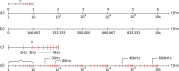
\includegraphics[width=\textwidth]{figure/scala_log_1.pdf}%
    \caption{Costruzione di una scala logaritmica}
    \label{fig:howtolog}
\end{figure}

Prendendo come riferimento l'unità di misura \hlight{$u$} stabilita, si segnano sulla parte superiore dell'ascissa i valori che vanno da $0$ a $6$ e, in corrispondenza di ognuno di essi, gli argomenti dei logaritmi che li hanno \textit{generati}, ovvero le frequenze che vanno da $1\Hz$ a $1\MHz$.

Per confronto si osservi invece l'ascissa di figura~\ref{fig:howtolog}\maroon{b} ricavata dividendo semplicemente in sei parti uguali il limite superiore del range di frequenza. In corrispondenza dei $10\Hz$ della scala logaritmica si hanno $166.667\Hz$ su quella lineare, in corrispondenza dei $1000\Hz$ di quella logaritmica si arriva a ben $500.000\Hz$ (cinquecentomila) su quella lineare.

I valori più bassi di frequenza della scala logaritmica subiscono, fino a poco più di metà range, un'espansione che poi man mano si comprime permettendo così di leggere cosa accade proprio in quelle frazioni di frequenza iniziali.

Naturalmente anche le porzioni intermedie di frequenza dovranno essere tracciate su scala logaritmica. Si prenda allora come riferimento la porzione di frequenza della 
figura~\ref{fig:howtolog}\maroon{a} che va da $1\Hz$ a $10\Hz$ che si è stabilito essere pari all'unità di misura \hlight{$u$} e che corrisponda per esempio a $25\mm$.

Al logaritmo di $1\Hz$ corrisponde come già detto il valore $0$, mentre al logaritmo di $10\Hz$ corrisponde il valore $1$.

Ciò che occorre fare, è calcolare i valori dei logaritmi intermedi che vanno da $2\Hz$ a $9\Hz$ che, moltiplicati per l'unità di misura \hlight{$u=25\mm$}, forniranno la distanza delle tacche dall'origine:
%%
\begin{align*}
 p_1 &= \log(2)*25 = 7,5\mm & p_2 &= \log(3)*25 = 11,9\mm & p_3 &= \log(4)*25 = 15,1\mm \\
 %%
 p_4 &= \log(5)*25 = 17,5\mm & p_5 &= \log(6)*25 = 19,5\mm & p_6 &= \log(7)*25 = 21,1\mm \\
 %%
 p_7 &= \log(8)*25 = 22,6\mm & p_8 &= \log(9)*25 = 23,9\mm & &
\end{align*}
%%
dove $p_1, p_2, \ldots, p_8$ sono le distanze delle singole tacche dall'origine. Si ottiene quindi la suddivisione mostrata in figura~\ref{fig:howtolog}\maroon{c} (scalata il doppio per mettere in evidenza la suddivisione) che, riportata intervallo dopo intervallo sull'asse delle ascisse di figura~\ref{fig:howtolog}\maroon{a}, suddivide infine l'ascissa logaritmica come in figura~\ref{fig:howtolog}\maroon{a}.

I diagrammi logaritmici dove uno degli assi è graduato linearmente sono detti \hlightit{semilogaritmici} (abbreviate anche come \hlightit{lin-log}); quelli in cui uno degli assi è invece espressione di valori calcolati con funzioni logaritmiche, sono invece detti \hlightit{bilogaritmici} (\hlightit{log-log}, vedi figura~\ref{subfig:filtro_log} dove l'ordinata destra è l'attenuazione espressa in $\decibel$).


					\subsection{Caratteristiche di un grafico}

Molto spesso, specie per la misura di grandezze fisiche affette da errori sistematici, è utile rappresentare non solo le curve o le spezzate definite da dati calcolati o dalle misure eseguite, ma anche gli errori ad esse correlate come in figura~\ref{fig:errori}
%%
\begin{figure}[ht!pb]
\centering
    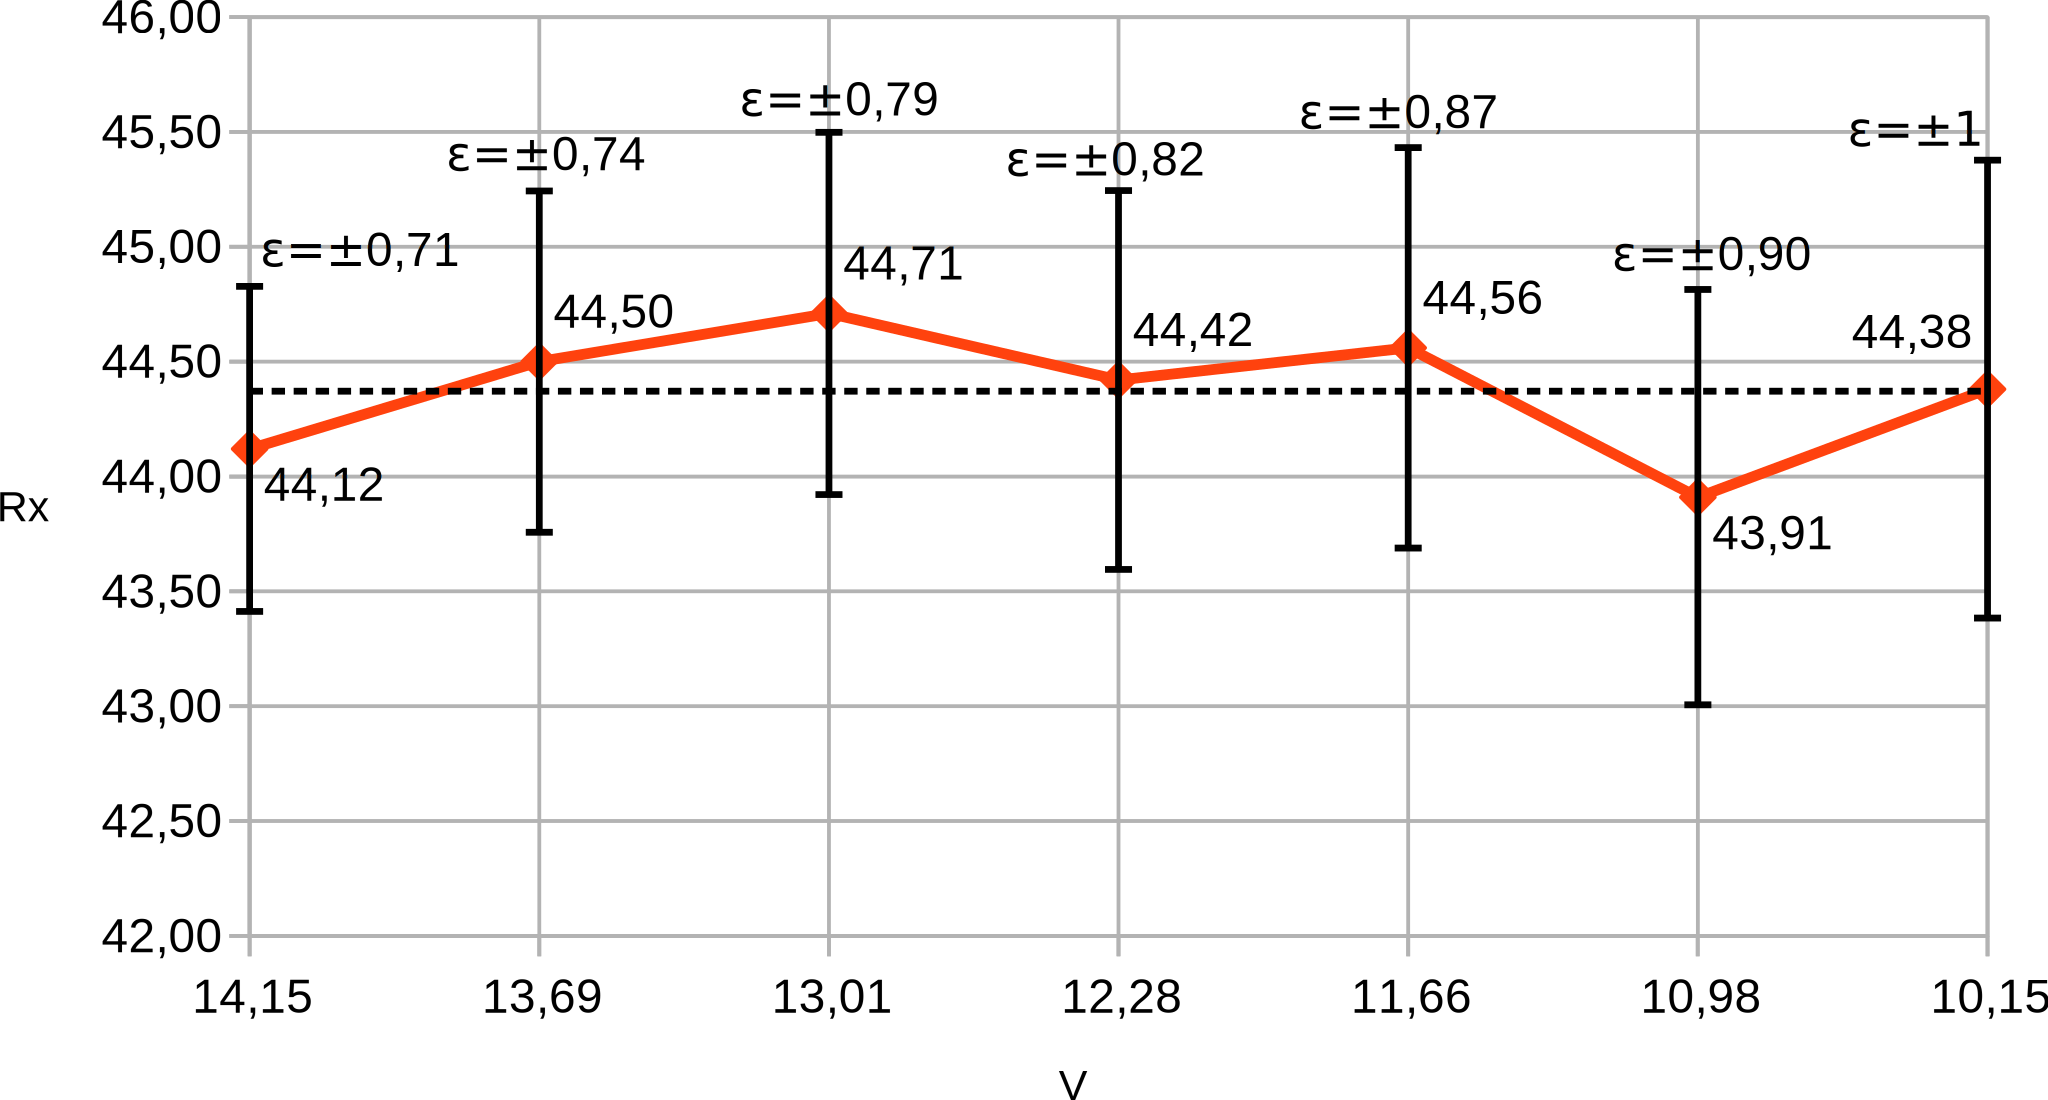
\includegraphics[width=0.8\linewidth]{figure/resistenza_con_errore.pdf}%
    \caption{Caratteristica di una curva in cui sono messi in evidenza gli errori $\eass$.}
    \label{fig:errori}
\end{figure}
%%
dove punto per punto, misura per misura, sono messe in evidenza le \textit{incertezze} (linee verticali).

Non di rado può essere utile rappresentare gli andamenti dei valori massimi e minimi delle misure in modo da mettere in evidenza il \textit{tunnel} entro cui si muove il valore centrale.

Le linee verticali vengono dette \hlightit{barre di errore} e indicano un intervallo di \textit{confidenza} o \textit{incertezza} (ovvero l'errore) relativo alle misure.

Il modo con cui i dati vengono visualizzati non è questione da poco, 
%%
\begin{figure}[htp]
	\centering
	\subfloat[Spezzate che uniscono i punti delle misure.]{%
		\includegraphics[width=0.5\textwidth]{figure/grafico_resistenza.pdf}\label{subfig:caratt_graph_a}%
	}
\hfill
	\subfloat[Linee descritte tramite interpolazione lineare.]{%
		\includegraphics[width=0.5\textwidth]{figure/interpolazione_polinomiale_resistenza.pdf}\label{subfig:caratt_graph_b}%
	}
	\caption[Caratteristiche delle linee di un grafico.]{Caratteristiche delle linee di un grafico: tramite spezzate o tramite interpolazione lineare.}
	\label{fig:caratt_graph}
\end{figure}

Per esempio, i punti della figura~\ref{subfig:caratt_graph_a} sono uniti tra loro da spezzate che, insieme, danno luogo all'\hlightit{interpolazione lineare}. Tale costruzione grafica non permette però di determinare in maniera efficace e men che meno precisa (al netto dell'errore comunque esistente) cosa accade nei punti intermedi.

Altro modo di rappresentare lo stesso insieme di tati è quello di ricorrere all'\hlightit{interpolazione polinomiale} in modo da descrivere, tramite curve e se possibile, il probabile valore di punti che non appartengono all'insieme dei dati misurati (figura~\ref{subfig:caratt_graph_b}).



					\section{Il luogo dei dati: le tabelle}

Una tabella è uno schema organizzato per righe e per colonne in cui inserire informazioni secondo un determinato criterio.

Le tabelle, quando unite a una efficacie rappresentazione grafica, sono uno degli strumenti più potenti con cui mostrare e riassumere gruppi correlati di dati.

Le informazioni provenienti da misure prese sul campo o elaborate attraverso analisi successive, possono essere così numerose che il loro uso nel testo o in formule ripetitive, possono determinare più confusione che chiarezza.

Raccogliere quindi tali informazioni in strumenti come tabelle, rende più facile e meno \textit{ingombrante} la lettura del testo.

Non va infatti dimenticato che una relazione, specie se tecnico-scientifica, deve godere di otto proprietà:
%%
\begin{enumerate}
 \item autorevolezza sulla modalità con cui vengono raccolti i dati e loro qualità;
 %%
 \item descrizione tecnicamente e grammaticamente inconfutabile;
 %%
 \item uso di un numero di pagine strettamente necessario;
 %%
 \item uso di adeguate teorie e formulazione di appropriate ipotesi;
 %%
 \item uso di adatti metodi per la misura del o dei fenomeni che si stanno osservando;
 %%
 \item uso appropriato di formule e grafici;
 %%
 \item analisi dei dati e verifica delle ipotesi;
 %%
 \item deduzioni e conclusioni.
\end{enumerate}

Un tabella diventa efficace se ben progettata e se possiede una struttura che consenta di leggere facilmente le singole informazioni. Una delle difficoltà maggiori consiste nel saper riconosce i dati che vanno organizzati per righe e per colonne e se, eventualmente, non sia il caso di dividerli in più tabelle.

Una tabella deve essere sempre identificata da una descrizione --la \hlightit{didascalia}-- che, al contrario delle figure, va posta sempre in alto. Come giù detto per le figure, la didascalia è bene che venga preceduta da un prefisso e da un numero consecutivo, con cui poterla identificare e richiamare in altre parti del testo (per esempio \maroon{Tab.\,1}, \maroon{Tabella\,1}, \maroon{Tab.1.2}, \ecc).


				\subsection{Struttura di una tabella}

Come accennato una tabella non è altro che una matrice formata da righe e colonne. In corrispondenza di ogni intersezione riga-colonna, detta \hlight{cella}, viene posto il dato.

La struttura più classica e completa di una tabella è quella di figura~\ref{fig:tab_index}
%%
\begin{figure}[htp!b!]
\centering\small
    \tabindice
    \caption{Parti di una tabella.}
    \label{fig:tab_index}
\end{figure}
%%
dove si riconosce una \hlightit{colonna indice} e un elenco di voci dette \hlightit{entrate} che indicizzano le colonne successive appartenenti a una stessa riga. Un banale esempio di colonna indice è la tabella~\ref{tab:tabindex} dove la prima colonna indica il numero della prova a cui i valori presenti nelle colonne seguenti si riferiscono.
%%
\begin{table}[h!tp]
 \centering\small
 \caption{Esempio di una tabella con colonna indice.}
 \tabesempioaA
 \label{tab:tabindex}
\end{table}

L'indicizzazione diventa utile nei casi in cui occorra riferirsi a uno o più valori ottenuti nel corso di una determinata misura.

Quando si progetta una tabella, le prime righe in alto sono sempre occupate dalle \hlightit{intestazioni} che specificano la natura della colonna e quindi dei dati posti nelle righe seguenti%%
%%
			\footnote{Nella tabella~\ref{tab:tabindex}, le intestazioni specificano che i valori presenti nelle righe che seguono sono letture di tensione, corrente o quelli della resistenza calcolata.}.
%%
Le intestazioni come quelle della tabella~\ref{tab:tabindex}, \textit{Voltometro} e \textit{Amperometro}, possono anche estendersi su più di una colonna quando, le informazioni contenute su più di una colonna, interessano un comune strumento, una comune grandezza, un comune fenomeno o altro ancora.

Nel caso in cui l'intestazione definisca grandezze fisiche, occorre anche specificare l'unità di misura, facendo eventualmente ricorso a opportuni multipli o sottomultipli, a cui i valori delle righe che seguono si riferiscono. In questo modo si evita non solo di dover ripetere per ogni valore l'unità di misura, ma anche l'inutile ripetizione di una informazione che appesentirebbe, specie nelle tabelle strutturalmente più complesse, la lettura.

Nel caso in cui il dato di una determinata cella non sia disponibile, al suo posto vengono inseriti tre punti o tre trattini.


					\subsection{Filetti, linee e griglie di una tabella: orrori da evitare}

Molti sono pronti a credere che una tabella sia effettivamente tale, solo se righe e colonne vengono delimitate da \hlightit{filetti} (\textit{linee}) verticali e orizzontali come nella tabella~\ref{tab:grigliata}.
%%
\begin{table}[htp]
 \centering\small
 \caption{Tabella con griglia. Errore da evitare.}
 \tabgrigliata
 \label{tab:grigliata}
\end{table}

Tabelle simili, specie se composte da un numero non indifferente di righe e colonne, sono assolutamente da evitare perché affaticano la vista e rendono le tabelle stesse meno leggibili.

Si crede infatti che il miglior modo per separare un dato da un altro, sia il tratto di linea che delimita e confina le informazioni contenute nelle singole celle.

L'alternativa esiste ed è quella paradossalmente ritenuta meno plausibile: usare pochissimi tratti di linea. Si confronti la grafica della tabella~\ref{tab:tabindex} a pagina~\pageref{tab:tabindex}, con quella della tabella con griglie. Leggera e più leggibile la prima, pesante e soffocante l'altra.

Con tre sole linee orizzontali si è dato alla tabella un aspetto graficamente e tipograficamnete migliore: due linee delimitano in alto e in basso la tabella, una terza linea, di spessore minore, separa invece le intestazioni dalle righe contenenti i dati.

Naturalmente il numero delle linee da utilizzare varia in base alla complessità della tabella. Come mostrato nella tabella~\ref{tab:tabindex}, altre due linee vengono utilizzate per delimitare, orizzontalmente, le intestazioni relative al \textit{Voltometro} e all'\textit{Amperometro}. La regola è: non esiste una regola se non quella di evitare assolutamente tabelle \textit{grigliate}.

Per dare il senso di alternanza delle righe di una tabella, si può utilizzare l'escamotage di colorare alternativamente le righe con un tenue punto di grigio in modo da migliorare, per così dire, la selettività visiva delle informazioni come in tabella~\ref{tab:alternata}.
%%
\begin{table}[htp]
 \centering\small
 \caption[Tabella con righe colorate alternativamente.]{Tabella con righe colorate alternativamente. Viene mantenuta la leggerezza grafica della tabella e contemporaneamente si è aumentata la distanza visiva tra una riga e un'altra senza l'uso di linee orizzontali.}
 \tabalternata
 \label{tab:alternata}
\end{table}

Si raccomanda, a meno di esigenze o richieste tipografiche particolari e tipiche comunque delle brochure o di documenti \textit{patinati}, l'uso di colori in tinta grigia chiara. Colori quali il rosso, il blu o anche il verde (ritenuto visivamente riposante, rischiano di affaticare la vista e di affogare le informazioni in inutili \textit{scale cromatiche}.

Una tabella  può naturalmente essere anche predisposta per raccogliere non solo informazioni di tipo numerico, ma anche informazioni prevalentemente testuali o grafiche (per esempio una tabella destinata a raccogliere la simbologia utilizzata in un particolare documento).

Un esempio è dato dalla tabella~\ref{tab:testuale} dove la colonna indice viene utilizzata per definire i periodi geologici. Trattandosi pur sempre di una tabella che per definizione assolve alla funzione di prospetto riassuntivo, la lunghezza del testo deve essere limitata a quella strettamente necessaria.
%%
\begin{table}[htp]
 \centering\small
 \caption[Tabella testuale.]{Tabella testuale. Si noti la possibilità di spezzare le linee di testo presenti in ciascuna cella.}
 \tabtestuale
 \label{tab:testuale}
\end{table}









						\section{Citazioni, note e bibliografia}

Scrivere un documento significa anche attingere ad altri tipi di informazioni, studi precedenti come anche a esperienze di altro genere. Potrebbe quindi nascere la necessità di doversi riferire a uno o più articoli, report, analisi, studi o norme che possono essere citati più volte e in più modi.

In questi casi il testo può essere riportato sia nel \hlightit{corpo del testo} sia \hlightit{fuori testo}. Si adotta il primo metodo nel caso in cui il testo da citare sia relativamente breve, il secondo modo se la citazione è ben più complessa ed estesa.

Nel caso di una citazione nel corpo, il testo dovrà essere messo in evidenza (solitamente si usa lo stile \textit{corsivo}) e sarà delimitato da virgolette (i cosiddetti \hlightit{caporali} 
<<\ldots~testo~\ldots>>) come l'esempio che segue:

\begin{quote}\small
[\ldots]~Lo studio delle leggi che formano il nucleo della meccanica classica e di quelle sulla gravitazione, non può che ricondursi a Isaac Newton che, proprio sulla forza di gravità e della luna scrisse: <<\emph{Cominciai a pensare che la forza di gravità potesse estendersi all'orbita della Luna}>>[\ldots]
\end{quote}

Nel caso di citazioni fuori dal corpo, il testo viene scritto su una paragrafo a parte. Per dare maggiore enfasi alla citazione e per non rischiare di confonderla con il testo che la ospita, si utilizza un \hlightit{paragrafo rientrato} e un testo con un corpo più piccolo:

\begin{quote}\small
[\ldots]~il calcolo delle correnti di cortocircuito nelle reti alimentate a bassa tensione, deve tener conto di quanto stabilito dalla norma \textsc{cei 11-28} (\textit{Guida d'applicazione per il calcolo delle correnti di cortocircuito nelle reti radiali a bassa tensione}) che definisce il corto circuito come:
%%
		\vspace{-5pt}\begin{changemargin}{5mm}{5mm}\footnotesize
      Connessione accidentale o intenzionale, di resistenza o impedenza relativamente bassa, di due o più punti in un circuito che normalmente sono a tensione diversa (IEV, Pubblicazione IEC 50 151-03-41 Chapter 151: Electrical and magnetic devices).
		\end{changemargin}
\end{quote}\vspace{-5pt}

Si noti l'uso di un paragrafo separato e il corpo del font più piccolo.

Un aspetto di fondamentale e deontologica correttezza e importanza è, nel caso si faccia uso di citazioni, di studi o analisi provenienti da altri, come anche parti di testo prese integralmente da articoli o altro, è l'indicazione delle fonti.

Le frazioni di testo prese da supporti cartacei o digitali o provenienti dal web o da altri metodi di trasmissione, anche se sommariamente rielaborate con il ricorso di sinonimi, devono essere accompagnate da note in cui viene specificato l'autore o gli autori, i lavori a cui ci si è ispirati, il titolo dell'opera, l'\textsc{url} dell'articolo eccetera. In caso contrario si commette un abuso che non consiste solo nel millantare idee non proprie, ma di consumare un reato accademicamente ben più grave: il \hlightit{plagio}.

L'Università di Pisa definisce il plagio nel seguente modo:

                  \begin{quote}
										[il plagio] è definito come la parziale o totale attribuzione di idee, ricerche o scoperte altri a se stessi o ad un altro autore, a prescindere dalla lingua in cui queste sono ufficialmente presentate o divulgate, o nell'ommissione della citazione delle fonti.
                  \end{quote}

L'indicazione della fonte può seguire la citazione o essere specificata in una nota a piè di pagina o a margine del testo. A tali modi si preferisce, se possibile e specie se il numero delle citazioni o dei riferimenti a altri lavori diventa importante, l'usi della \hlightit{bibliografia} inserita in una sezione a parte e a fine dell'elaborato.

I modi con cui citare un particolare elaborato o lavoro sono molti e dipendono anche dalla natura del testo che si sta scrivendo. (umanistico, tecnico-scientifico, filosofico, giuridico \ecc).

Una citazione bibliografica è composta dai seguenti elementi:

\begin{quotation}\small
 [<etichetta>] <autore o autori (in tondo)>. <\textit{Titolo} in \textit{corsivo}>. <Editore>, <anno di pubblicazione>, <codice \textsc{isbn}> (<pagina in cui compare la citazione>)
\end{quotation}

Per esempio:
%%
		\begin{quote}\small
			\begin{enumerate}[leftmargin=20mm]
				\item[$\textlbrackdbl$HS16$\textrbrackdbl$] M.~Hughes e B.~Sansone. \textit{Arduino per tecnici, ingegneri e maker}. Tecniche nuove, 2016. \textsc{isbn}: 9788848131780 (cit. a p.~4)
			\end{enumerate}
		\end{quote}

Se la citazione riguarda un'opera o un articolo disponibile su \textsc{web}, la citazione potrà essere scritta come:
%%
		\begin{quote}\small
			\begin{enumerate}[leftmargin=25mm]
				\item[$\textlbrackdbl$avrdude$\textrbrackdbl$] Systutorial. \textit{Linux Man Pages--averdude man page}. \url{https://www.systutorials.com/docs/linux/man/1-avrdude} (cit. a p.~13)
			\end{enumerate}
		\end{quote}
%%
e nel caso sia poi possibile scaricare un documento in formato elettronico:
%%
		\begin{quote}\small
			\begin{enumerate}[leftmargin=25mm]
				\item[$\textlbrackdbl$Plan$\textrbrackdbl$] PlatformIO. \textit{PlatformIO Documentation}. jun 25,2018. \url{https://media.readthedocs.org/pdf/platformio/latest/platformio.pdf} (cit. a p.~6)
			\end{enumerate}
		\end{quote}
%%
dove [HS16], [avrdude], [Plan] sono possibili etichette (in gergo \hlightit{label}) che compaiono nei punti in cui sono presenti le citazioni. Le label possono essere non solo alfabetiche, ma anche unicamente numeriche o alfanumeriche.


					\section{Conclusioni}

Scrivere una buona relazione, fosse anche un breve report, un articolo o saggio breve comporta inevitabilmente una buona, anzi ottima, conoscenza della materia o dei singoli argomenti che si stanno trattando (nei lavori di gruppo, i componenti potrebbero infatti essere esperti o competenti solo per una frazione del lavoro che si sta svolgendo).

Nel caso in cui il documento sia strutturato e composto da più di quindici-venti pagine contenenti grafici e tabelle, l'autore dovrà considerare la possibilità di inserire nelle prime pagine, un indice generale che elenca divisi per sezioni o eventualmente anche per sottosezione gli argomenti trattati e un indice delle figure e delle tabelle. Le pagine dovranno essere ovviamente numerate.

Si raccomanda anche di comporre in modo corretto la cosiddetta \hlightit{prima pagina di copertina} che dovrà comprendere nome e cognome dell'autore o degli autori, l'istituzione, azienda o altro di cui si fa parte, il titolo del documento, la data e, se possibile, un \hlightit{logo}.

Possibili \textit{prime di copertina} sono quelle indicate in figura~\ref{fig:fpage} a pagina~\pageref{fig:fpage}.

Una relazione dovrà essere strutturata e comprendere:
%%
\begin{enumerate}
 \item oggetto e scopo;
 %%
 \item schemi, disegni e tabelle;
 %%
 \item nel caso si faccia un uso esteso di una particolare simbologia o di acronimi, inserire in apertura una tabella dei simboli e una lista degli acronimi comprensivi di breve significato;
 %%
 \item eventuali definizioni date a termini tecnici;
 %%
 \item esposizione della teoria, delle ipotesi e dei modelli matematici o circuitali usati nel corso delle prove, misure, esperimento \ecc;
 %%
 \item calcoli preliminari e scelta degli strumenti le cui caratteristiche devono essere oggetto di una tabella a parte;
 %%
 \item condotta della prova, misure e, se richiesti o necessari, raccolta di altri dati ritenuti necessari (per esempio temperatura ambientale, tasso di umidità, \ecc);
 %%
 \item analisi dei dati e dei valori misurati, eventuale esclusione di dati ritenuti errati o incongruenti. La scelta dell'esclusione va in ogni caso motivata;
 %%
 \item definizione e spiegazione dei termini che compaiono nelle formule e calcoli. Nel caso in cui i calcoli siano numerosi e prodotti da un numero ristretto di formule continuamente reiterate, anziché ripeterli, si descriverà una sola volta il significato delle formule e dei termini che vi compaiono e si inseriranno i valori elaborati a parte, in una o più tabelle;
 %%
 \item analisi dei valori calcolati;
 %%
 \item conclusioni e deduzioni.
\end{enumerate}

\begin{landscape}
\begin{figure}[htp]
	\centering
%	\subfloat[Prima Pagina di copertina.]{%
		\includegraphics[width=0.65\textheight]{figure/frontpage_1.pdf}%
%	}
\hfill
%	\subfloat[<caption_fig2>]{%
		\includegraphics[width=0.65\textheight]{figure/frontpage_2.pdf}%
%	}
	\caption{Possibili prime pagine di copertina.}
	\label{fig:fpage}
\end{figure}
\end{landscape}































%%%%%%%%%%%%%%%%%%%%%%%%%%%%%%%%%%%%%%%%%%%%%%%%%%
%%%%%%%%%%%%%%%%%%%%%%%%%%%%%%%%%%%%%%%%%%%%%%%%%%
%%%%%%%%%%%%%%%% A P P E N D I C I %%%%%%%%%%%%%%%
%%%%%%%%%%%%%%%%%%%%%%%%%%%%%%%%%%%%%%%%%%%%%%%%%%
%%%%%%%%%%%%%%%%%%%%%%%%%%%%%%%%%%%%%%%%%%%%%%%%%%
%\appendici

%\input{appendici/platformio_board.tex}
%\input{appendici/avrdude.tex}

%\subsection{Lorem ipsum}
%\lipsum[6-7]
%%
%\subsection{kantlipsum}
%\kant[6-11]
%\end{multicols}

%\backmatter

%%%%%%%%%%%%%%%%%%%%%%%%%%%%%%%%%%%%%%%%%%%%%%%%%%
%%%%%%%%%%%%%%%%%%%%%%%%%%%%%%%%%%%%%%%%%%%%%%%%%%
%%%%%%%%%%%%% B I B L I O G R A F I A %%%%%%%%%%%%
%%%%%%%%%%%%%%%%%%%%%%%%%%%%%%%%%%%%%%%%%%%%%%%%%%
%%%%%%%%%%%%%%%%%%%%%%%%%%%%%%%%%%%%%%%%%%%%%%%%%%
\blankpage
\biblio
%\defbibheading{citata}{\subsection{Bibliografia citata nel testo}}
\defbibheading{approfondimento}{\subsection{Bibliografia di approfondimento}}
%%%%%%%%%%%%%%%%%%%%%%%%%%%%%%%%%%
%% Bibliografia Citata
%%%%%%%%%%%%%%%%%%%%%%%%%%%%%%%%%%
%\defbibheading{citata}{}
%\defbibheading{approf}{}
%\defbibnote{citata}{}
%\defbibnote{approf}{}
%\phantomsection
%\addcontentsline{toc}{subsection}{Bibliografia citata nel testo}%\nocite{*}
%\printbibliography[keyword={citata},heading={subbibliography}, title=Bibliografia citata nel testo]
%%%%%%%%%%%%%%%%%%%%%%%%%%%%%%%%%%
%% Bibliografia Non Citata
%%%%%%%%%%%%%%%%%%%%%%%%%%%%%%%%%%
\phantomsection
\addcontentsline{toc}{subsection}{Bibliografia di approfondimento}
\nocite{*}
\printbibliography[keyword={approf},heading={subbibliography}, title=Bibliografia di approfondimento]
%
%%%%%%%%%%%%%%%%%%%%%%%%%%%%%%%%%%%%%%%%%%%%%%%%%%
%%%%%%%%%%%%%%%%%%%%%%%%%%%%%%%%%%%%%%%%%%%%%%%%%%
%%%%%%%%%%%%%%%%%%% I N D I C E %%%%%%%%%%%%%%%%%%
%%%%%%%%%%%%%%%%%%%%%%%%%%%%%%%%%%%%%%%%%%%%%%%%%%
%%%%%%%%%%%%%%%%%%%%%%%%%%%%%%%%%%%%%%%%%%%%%%%%%%
%\blankpage
%\indice

%%%%%%%%%%%%%%%%%%%%%%%%%%%%%%%%%%%%%%%%%%%%%%%%%%
%%%%%%%%%%%%%%%%%%%%%%%%%%%%%%%%%%%%%%%%%%%%%%%%%%
%%%%%% Q U A R T A   DI   C O P E R T I N A %%%%%%
%%%%%%%%%%%%%%%%%%%%%%%%%%%%%%%%%%%%%%%%%%%%%%%%%%
%%%%%%%%%%%%%%%%%%%%%%%%%%%%%%%%%%%%%%%%%%%%%%%%%%
% Sintassi:
% \quartadicopertina{testo_qr|url}{0|1}{<testo_quarta_copertina>}
% Se il primo valore passato è = 0 non viene composto il codice a barre
% SE il secondo valore è = 0 il QR non ha link, se invece è = 1 viene composto come link
\quartadicopertina{http://www.marconicivitavecchia.it}{1}{MarconiInstitutePress}%ManualiAbImis

\end{document}


%%%%%% INSERIRE FIGURA NELLA COLONNA:

\begin{figure}[H]%[htb!] %option=htb
\centering
    \includegraphics[width=0.8\linewidth]{figure/braccio_meccanico_small.png}%
    \caption{Braccio meccanico realizzato nel fablab.}
    \label{fig:uno}
\end{figure}

%%%%%% INSERIRE FIGURA A LARGHEZZA PAGINA:

\figtwocol{htbp!}{<num_tra_0_e_1>}{<path>/<nome_file>}{<caption>}{<label>}

